% First TeX Draft für Fabi's Diss. Adapted from Tobi's texfile
\documentclass[twoside,10pt,openright]{scrbook} % right-side equation numbering, 10 point font, print two-sided, chapterbegin on the right

\KOMAoptions{BCOR=16mm,  	%
 	     DIV=12,		%
	     twocolumn=false, 	%
	     paper=A4, 		%
	     draft=false,	%
	     titlepage=true,	%
	     toc=listof,	%
	     headsepline=true,	%
	     footsepline=false,
	     toc=bibliography,
	     numbers=noendperiod}

\usepackage[default]{lato}
\usepackage{amsxtra}     % Use various AMS packages
\usepackage{amsthm}
\usepackage{amssymb}
\usepackage{amsfonts}
\usepackage{mathpazo}
\usepackage{graphicx}    % Add some packages for figures. Read epslatex.pdf on ctan.tug.org
\usepackage{caption}    % Add some packages for figures. Read epslatex.pdf on ctan.tug.org
\usepackage{rotating}
\usepackage{color}
\usepackage{epsfig}
\usepackage{subfigure}   % To make subfigures. Read subfigure.pdf on ctan.tug.org
\usepackage{verbatim}
\usepackage{natbib}      % Allows you to use BibTeX
\usepackage{setspace}    % Allows you to specify the line spacing
\usepackage{parskip}	 % no indent
\usepackage{fancyhdr}
\usepackage{tabularx}
\usepackage{nomencl}
\usepackage{lscape}
\usepackage[utf8]{inputenc} % to be sure
\usepackage{csquotes}
\usepackage{index}
\usepackage{float}
\usepackage{pdfpages}
\usepackage{textcomp} % \textcelsius
\usepackage{nth}
\usepackage{enumerate}
\usepackage{enumitem}
\usepackage{cclicenses}
\usepackage{wrapfig}
\usepackage{minted}
\usepackage{hanging}
\usepackage{bbding}
\usepackage{microtype}
%\usepackage[section]{placeins} this was to force figures to section. in the end maybe
\usepackage{placeins}
\usepackage[usenames,dvipsnames]{xcolor}
\usepackage[toc,page]{appendix}
\usepackage{perpage} %the perpage package
\MakePerPage{footnote} %the perpage package command
\usepackage{float}



\usepackage[bookmarks,colorlinks,citecolor=MidnightBlue,urlcolor=MidnightBlue,linkcolor=MidnightBlue,hypertexnames=false]{hyperref}
%\usepackage[bookmarks,colorlinks,citecolor=Black,urlcolor=Black,linkcolor=Black,hypertexnames=false]{hyperref}

\newcommand{\HRule}{\rule{\linewidth}{0.5mm}}
%\renewcommand*{\thefootnote}{\fnsymbol{footnote}}
%\newcommand\HUGE{\@setfontsize\Huge{38}{47}} 

\newcommand{\figs}{../habil/img}

%\doublespacing %gonehalfspacing for 1.5 spacing, \doublespacing for 2.0 spacing.
\onehalfspacing

\author{Fabien Maussion}
\title{Numerical modelling of \\ global glacier change}
\subtitle{}
\date{2021}

\makeatletter
\def\thickhrulefill{\leavevmode \leaders \hrule height 1pt\hfill \kern \z@}
\renewcommand{\maketitle}{\begin{titlepage}%
  
	\begin{center}
		% Upper part of the page
	  	\vspace*{0cm}
		\Huge \bfseries \MakeUppercase{\@title} \mdseries \\[1.5cm]
				
		\Large \MakeUppercase{Habilitation thesis} \\	[1cm]		
		\Large Fabien Maussion \\	[0.1cm]		
		\large 2021 \\ [4.5cm]

		\begin{figure}[h!]
		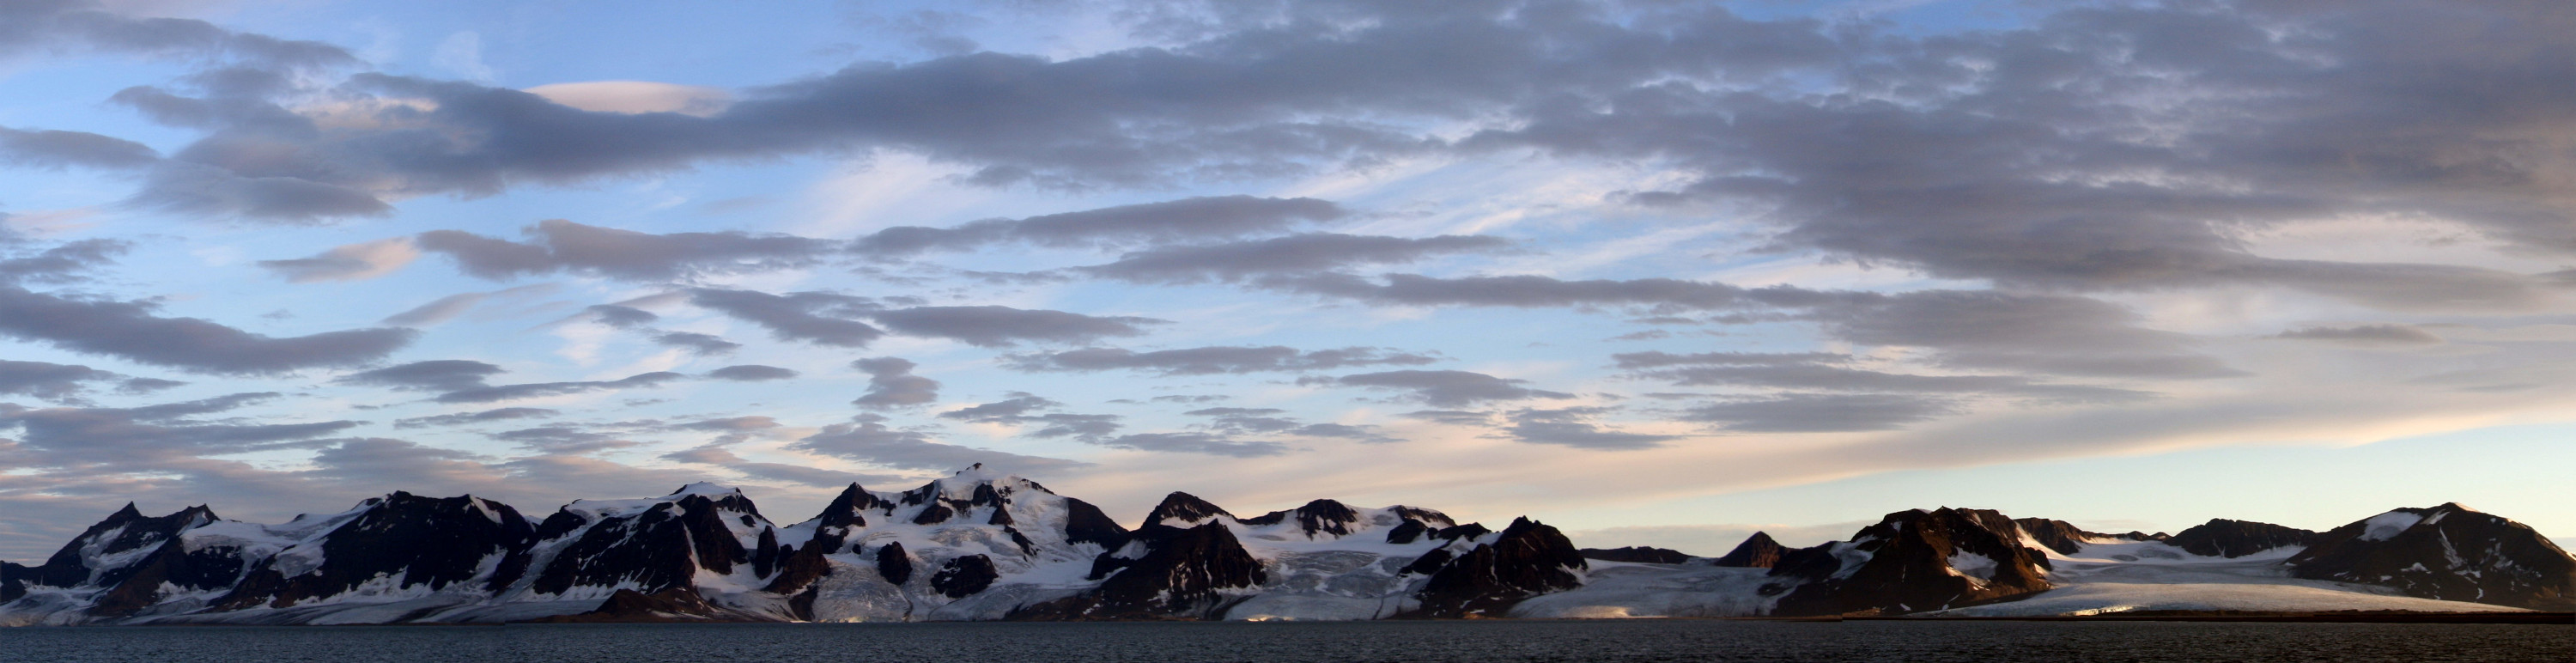
\includegraphics[width=\textwidth ,angle=0]{\figs/title_pic.jpeg} \\ [3cm]
		\end{figure}

		\large Submitted to the Faculty of Geo- and Atmospheric Sciences \\ at the University of Innsbruck, Austria.
	\end{center}
        %\large Institut für Ökologie \\[0.2cm]
        %\large Fachgebiet Klimatologie \\[1.2cm]  
		%\large Dr. rer. nat. \\[1.2cm]
  \end{titlepage}%
  \setcounter{footnote}{0}%
}
\makeatother


%----------------------------------------------------
% Chapter  style
%----------------------------------------------------
\makeatletter
\def\@makechapterhead#1{%
  \vspace*{50\p@}%
  {\parindent \z@ \raggedleft \normalfont
    \ifnum \c@secnumdepth >\m@ne
      \if@mainmatter
      \Large \@chapapp\space \Huge\thechapter
        \par\nobreak
        \vskip 40\p@
      \fi
    \fi
    \interlinepenalty\@M
    \hrule
    \vspace*{12\p@}%
    \huge #1\par\nobreak
    \par
    \vspace*{20\p@}%
    \hrule
    \vskip 50\p@
  }}
\def\@schapter#1{\if@twocolumn
                   \@topnewpage[\@makeschapterhead{#1}]%
                 \else
                   \@makeschapterhead{#1}%
                   \@afterheading
                 \fi}
\def\@makeschapterhead#1{%
  \vspace*{50\p@}%
  {\parindent \z@ \raggedleft
    \normalfont
    \interlinepenalty\@M
    \hrule
    \vspace*{6\p@}%
    \Large #1\par\nobreak
    \par
    \vspace*{15\p@}%
    \hrule
    \vskip 40\p@
  }}
\makeatother

%-----------------------------------
% Header top/bottom
%-----------------------------------
\pagestyle{fancy}

%\renewcommand{\chaptermark}[1]{%
%\markboth{\MakeUppercase{%
%\chaptername}\ \thechapter.%
%\ #1}{}}
%\renewcommand{\chaptermark}[1]{\markboth{{\thechapter} #1}{}}
%\renewcommand{\sectionmark}[1]{\markright{{\thesection} #1}{}}

\renewcommand{\headrulewidth}{0pt}% Remove header rule
\fancyhead{}% Remove all header contents

%\definecolor{cadet}{RGB}{54,100,139}
%\definecolor{cadet}{RGB}{96,123,139}
%\definecolor{cadet}{RGB}{67,84,112}
%\fancyhead[]{}
%\fancyhead[RO]{{\rightmark}} % clear all header fields
%\fancyhead[LO]{}
%\fancyhead[LE]{{\leftmark}}
%\fancyhead[RE]{}
\fancyfoot{} % clear all footer fields
\fancyfoot[LE,RO]{\thepage}
\fancyfoot[LO,RE]{}
%\renewcommand{\headrulewidth}{0.4pt}
%\renewcommand{\footrulewidth}{0.4pt}

%----------------------------------
% Textauszeichnungen
%----------------------------------
\addtokomafont{captionlabel}{\footnotesize\bfseries}
\addtokomafont{caption}{\footnotesize}
\addtokomafont{section}{\Large}
\addtokomafont{subsection}{}
\addtokomafont{subsubsection}{}

\newif\iflong

\begin{document}

\setcounter{tocdepth}{1}

% Titleblatt einfügen
\maketitle

\frontmatter
\addchap{Preface}


This habilitation thesis consists of 13 peer reviewed publications completed
between 2015 and 2020. It also contains two short, previously unpublished chapters
introducing what I believe to be my most important contributions to the field of
large-scale glaciology to date: (i) the \href{https://oggm.org}{Open Global Glacier Model (OGGM)},
an open-source glacier evolution model, and (ii) \href{https://edu.oggm.org}{OGGM-Edu},
a collaborative educational website about glaciers. All papers, web platforms
and software presented here were prepared while I was working at the University of Innsbruck.

This thesis addresses several aspects of the numerical modelling of glacier change,
at various spatial (glacier to global) and temporal (annual to centennial) scales. Thanks to
the projects I had the chance to contribute to, it also develops some aspects of observational
glaciology and meteorology. However, the main bulk of this work is focussing on the central
topic of this thesis: \textbf{the development of modern numerical methods to (i) estimate the ice
thickness of mountain glaciers and their volume, (ii) compute their mass balance and (iii)
simulate their evolution under climate change}.

A further important theme that is developed in this thesis is the topic of \textbf{open science}.
Because of my personal conviction that all scientific results should be openly available, I have
spent a lot of thought and energy on developing methods and workflows that enable a more open,
accessible, documented, and reproducible scientific practice. Many of these ideas are not from my
own invention, but are workflows that I borrowed and adapted from the open-source software
development community.

All the work presented here is the result of numerous collaborations, within the University of Innsbruck,
but also originating from a wider network of collaborators and from international working groups.
Five of these papers arose from my contributions
to the doctoral studies of Beatriz Recinos and Julia Eis (University of Bremen), Ben Pelto (University of
Northern British Columbia), Stephan Galos (University of Innsbruck) and the master thesis of
Tobias Zolles (University of Innsbruck). \\ [0.8cm]

\textit{This thesis is also available as a website:}
\href{https://fabienmaussion.info/habil2.0}{www.fabienmaussion.info/habil2.0} \\
\textit{The content is strictly the same - readers are free to choose which format suits them better!}

\section*{Copyright notice}

All content in this thesis (except the linked publications) is licensed 
under a \href{https://creativecommons.org/licenses/by/4.0}.

The following papers are published with an open creative commons license:
01, 02, 04, 05, 06, 07, 08, 10, 11, 12. \\
The following papers are protected under publisher copyright: 03, 09, 13.

In order not to violate any copyright protection laws, the following documents have been generated:
\begin{itemize}
\item the online version of this thesis and the pdf available for download only link to the publisher's 
      version of the papers. This may lead you to a paywall for papers 03, 09, 13.
\item the pdf version sent to the reviewers contains all papers.
\end{itemize}


\cleardoublepage
\renewcommand*\contentsname{Table of contents}
\currentpdfbookmark{Table of contents}{name}
\tableofcontents

\mainmatter

% Do pdfs or not 
% \longtrue 
\longfalse

\chapter{Introduction}
\label{chap1}


My first “first-hand encounter” with the dramatic retreat of glaciers happened when I was 19, as I had to step down the
several ladders leading to the Mer de Glace in the region of Chamonix. These ladders allowed hikers to reach the glacier
from the Montenvers train station. In 2003, they were several dozens of meters long; they have been constantly
lengthened since then, to compensate for further glacier retreat \citep{Mourey2017}.

Beyond this sentimental aspect, glaciers have important societal impacts. They are contributing to sea-level rise, are
regulators of freshwater availability in many regions of the world, and they are sources of geohazards. Their documented
past fluctuations are a useful (but complex) recorder of past climates.

For all these reasons, mountain glaciers have been studied for centuries. More recently, the Intergovernmental Panel on
Climate Change (IPCC) published
a \href{https://www.ipcc.ch/srocc/}{Special Report on the Ocean and Cryosphere in a Changing Climate} (SROCC, 2019). It draws
a grim picture of the state of the cryosphere: I quote below parts of the summary for policy makers of Chapters 02
\citep{Hock2019a} and 04 \citep{Oppenheimer2019}.

\begin{quote}
\textit{Mass change of glaciers in all mountain regions (excluding the Canadian and Russian Arctic, Svalbard, Greenland and Antarctica) was very likely -490 \(\pm\) 100 kg m\(^{-2}\) yr\(^{-1}\) (-123 \(\pm\) 24 Gt yr\(^{-1}\)) in 2006--2015. Regionally averaged mass budgets were likely most negative (less than -850 kg m\(^{-2}\) y\(^{-1}\)) in the southern Andes, Caucasus and the European Alps/Pyrenees, and least negative in High Mountain Asia (-150 \(\pm\) 110 kg m\(^{-2}\) yr\(^{-1}\)) but variations within regions are strong.}
\end{quote}

\begin{quote}
\textit{Snow cover, glaciers and permafrost are projected to continue to decline in almost all regions throughout the 21st century (high confidence). (…) Projected glacier mass reductions between 2015--2100 are likely 22--44\% for RCP2.6 and 37--57\% for RCP8.5. In regions with mostly smaller glaciers and relatively little ice cover (…), glaciers will lose more than 80\% of their current mass by 2100 under RCP8.5 (medium confidence), and many glaciers will disappear regardless emission scenario (very high confidence).}
\end{quote}

\begin{quote}
\textit{Changes in snow and glaciers have changed the amount and seasonality of runoff in snow-dominated and glacier-fed river basins (very high confidence) with local impacts on water resources and agriculture (medium confidence). (…) In some glacier-fed rivers, summer and annual runoff have increased due to intensified glacier melt, but decreased where glacier melt water has lessened as glacier area shrinks. Decreases were observed especially in regions dominated by small glaciers, such as the European Alps (medium confidence).}
\end{quote}

\begin{quote}
\textit{River runoff in snow dominated and glacier-fed river basins will change further in amount and seasonality in response to projected snow cover and glacier decline (very high confidence) with negative impacts on agriculture, hydropower and water quality in some regions (medium confidence). (…) Projected trends in annual runoff vary substantially among regions, and can even be opposite in direction, but there is high confidence that in all regions average annual runoff from glaciers will have reached a peak that will be followed by declining runoff at the latest by the end of the 21st century.}
\end{quote}

\begin{quote}
\textit{Global mean sea-level (GMSL) is rising (virtually certain) and accelerating (high confidence). The sum of glacier and ice sheet contributions is now the dominant source of GMSL rise (very high confidence).}
\end{quote}

\begin{quote}
\textit{Future rise in GMSL caused by thermal expansion, melting of glaciers and ice sheets and land water storage changes, is strongly dependent on which Representative Concentration Pathway (RCP) emission scenario is followed. SLR at the end of the century is projected to be faster under all scenarios, including those compatible with achieving the long-term temperature goal set out in the Paris Agreement. GMSL will rise between 0.43 m (0.29--0.59 m, likely range; RCP2.6) and 0.84 m (0.61--1.10 m, likely range; RCP8.5) by 2100 (medium confidence) relative to 1986--2005.}
\end{quote}

The IPCC reports condense the results of decades of research, integrating a wealth of observational and modelling
studies at local, regional, and global scales. Such quantitative observations and projections of glacier change at large
scales have, for long, been possible only thanks to the use of ingenious upscaling methods to compensate for the limited
available data. By combining observations, modelling and rough estimates of glaciated area, pioneering studies helped to
quantify the contributions of glaciers and ice-caps to sea-level rise
\citep{Gregory1998,Raper2000,Wal2001,Braithwaite2002,Kaser2006a,Raper2006a,Meier2007,Cogley2009,Bahr2009}, providing
fundamental contributions to the 4th IPCC report on Climate Change (\href{https://www.ipcc.ch/report/ar4/wg1/}{AR4, 2007}).

However, the reputation of AR4 -- and, by extension, of the IPCC -- was damaged a few years later because of one
paragraph in the WG2 report (Ch. 10.6.2, “The Himalayan glaciers”), unrelated to the studies referenced here. This
paragraph wrongly stated that Himalayan glaciers were “likely to disappear by 2035”, despite being in contradiction with
the state of knowledge at that time \citep{Cogley2010}. The statement led to negative press for the IPCC and undermined its credibility as
a whole. Despite these long-lasting negative consequences, it is probable that this “Himalaya-gate” also led to an
increase of efforts from the mountain glacier research community towards more quantitative assessments of the state of
glaciers and their change, as well as an improved communication about the role of glaciers for downstream hydrology
\citep{Kaser.etal_2010,Radic2010,Radic2011,Bolch2012,Immerzeel2012}.

Motivated by the discrepancies of the few estimates and projections of global mass loss of glaciers available in AR4,
the first globally complete inventory of glaciers (the \href{https://www.glims.org/RGI}{Randolph Glacier Inventory, RGI}) was
produced to fulfill the needs of the forthcoming Fifth Assessment Report of the Intergovernmental Panel on Climate
Change (\href{https://www.ipcc.ch/report/ar5/wg1/}{IPCC AR5}). The RGI (a collection of glacier outlines complemented with
attributes such as glacier type, hypsometry, etc.) fundamentally changed the way that regional and global glacier change
assessments would be conducted \citep{Pfeffer2014}. One of the first observational study to make use of this inventory
was the “Reconciled Estimate of Glacier Contributions to sea-level Rise: 2003 to 2009” by 
\cite{Gardner2013}, and it was followed by many others \citep{Brun2017,Dussaillant2019,Shean2020}. The RGI also allowed
scientists to compute new estimates of global glacier volume, better constraining their potential contribution to
sea-level rise \citep{Huss2012,Grinsted2013}. Finally, the RGI paved the way for the development of a wealth of glacier
evolution models able to simulate the evolution of each glacier individually, making the use of upscaling strategies
more accurate or even obsolete
\citep{Marzeion2012,Giesen2012,Anderson2012,Giesen2013,Hirabayashi2013,Radic2014,Huss2015,Kraaijenbrink2017,Sakai2017,Shannon2019,Rounce2020}. 
Such models can be used to reconstruct past contributions of glacier to 20th century sea-level rise
\citep{Marzeion2015}, the part of past glacier loss due to anthropogenic causes \citep{Marzeion2014}, or the impact of
glacier change on future seasonal runoff in glaciated basins \citep{Bliss2014,Huss2018,Rounce2020b}, to cite only a few
of their many applications.

The work presented in this thesis is fully embedded in this global context. All studies presented here have been written
between 2015 and 2020, in between IPCC’s AR5 and the upcoming AR6. Several of them are originating from large
international collaborations, such as the working group
on \href{https://cryosphericsciences.org/activities/ice-thickness/}{Glacier ice thickness estimation} from the International
Association of Cryospheric Sciences (IACS), or the Glacier Model Intercomparison
Project (\href{https://www.climate-cryosphere.org/mips/glaciermip}{GlacierMIP}) from the Climate and Cryosphere (CliC) core
project of the World Climate Research Programme (WCRP).

Started in 2014, the development of the \href{https://oggm.org}{Open Global Glacier Model} (OGGM) could build upon the
experience gained from the pioneering studies listed above, and many others that could not be referenced here.
Benefiting from constantly improving observational datasets, the model is in continuous development to adapt for new
boundary conditions, or new datasets for calibration and validation. At the time of writing, OGGM is now an established
modelling framework, representing the “state-of-the art” in large-scale glacier modelling.

\section*{Synopsis of the thesis}
\addcontentsline{toc}{section}{\protect\numberline{}Synopsis of the thesis}%


This habilitation thesis summarizes a few of the many contributions to the tremendous progress made in the field of
large-scale gaciology since 2015. Of course, it is limited to my own contributions and only offers my personal perspective,
as is required for such a document. The thesis is organized around the following thematic chapters and publications:
\begin{itemize}[nosep]
\item {} 
In \textbf{Chapter 2}, I present the model description publication introducing OGGM, as well as several new developments
worth discussing here. OGGM is a modelling framework dealing with the entire glacier system, under several
simplifications required for large-scale applications. The following chapters therefore address three major aspects of
glacier system modelling.

\item {} 
In \textbf{Chapter 3}, I present four publications dealing with the topic of glacier ice thickness estimation using
numerical methods. Knowledge about glacier volume and bed topography is a prerequisite for the modelling of glacier
evolution.

\item {} 
In \textbf{Chapter 4}, I present four publications dedicated to glacier mass balance estimation, using in-situ and remote
observations combined with statistical and numerical methods. Surface mass balance is the most direct response of
glaciers to climate variations, and the observation of glacier mass balance provides invaluable calibration products
for glacier models.

\item {} 
In \textbf{Chapter 5}, I present four publications making use of the OGGM model to simulate past and future glacier change.
Two of them are focussing on the problem of reconstructing past glaciers length fluctuations, while the two others
deal with glacier change projections.

\item {} 
In \textbf{Chapter 6}, I introduce OGGM-Edu, an online educational platform about glaciers, built upon OGGM and for
high-school and university instructors.

\item {} 
In \textbf{Chapter 7}, I conclude this thesis and provide an outlook about planned future research based on OGGM.

\end{itemize}

Each thesis publication is preceded by a short introductions, meant to offer my personal
perspective on the content and genesis of the papers, as well as their relevance in the context
of this thesis.

I hope that you will enjoy this personal journey in the field of large-scale glacier modelling!

\chapter{The Open Global Glacier Model (OGGM)}
\label{chap2}


The Open Global Glacier Model (OGGM) is an open source modelling framework for glaciers. It has been developed since
2014: intermittently at first, and more regularly since 2016. Today, OGGM is continuously discussed and updated by a
team of researchers in various institutions.

“OGGM e.V” is a registered non-profit organization, which purpose is the promotion of science and research in the fields
of climate and glaciology; it does so by coordinating the development of OGGM and OGGM-Edu, and by organizing events
around the topic of large-scale glaciology.
\begin{itemize}
\item {} 
\textbf{Website:} \href{https://oggm.org}{https://oggm.org}

\item {} 
\textbf{Model documentation:} \href{http://docs.oggm.org}{http://docs.oggm.org}

\item {} 
\textbf{Online tutorials:} \href{http://oggm.org/tutorials}{http://oggm.org/tutorials}

\item {} 
\textbf{Source code:} \href{https://github.com/OGGM/oggm}{https://github.com/OGGM/oggm}

\item {} 
\textbf{Social media (twitter):} \href{https://twitter.com/OGGM\_org}{https://twitter.com/OGGM\_org}

\end{itemize}

Anyone can participate in the development of OGGM. In practice, however, the main bulk of development and funding effort
in the past have come from the Universities of Bremen (Ben Marzeion) and Innsbruck (myself). I have contributed to the
vast majority of the codebase, while strategic decisions have been shared between Ben and me, and in recent years with a
growing community of users.

This chapter briefly describes the OGGM project, its mission and building blocks. It concludes with a discussion about
some of the challenges the project is facing. For a discussion about the project’s future and long-term perspectives,
refer to Sect.~\ref{perspectives}.


\section{Objectives of the OGGM project}

The main mission of the OGGM project is to:

\begin{quote}
Develop a \textbf{global scale}, \textbf{modular}, and \textbf{open source} numerical model framework for \textbf{consistently} simulating past and future global scale glacier change
\end{quote}

\textbf{Global scale} means that OGGM should be applicable to all the world glaciers. This also means that it should be
applicable to a smaller ensemble of glaciers, for example at the catchment scale, or even one single glacier. However,
OGGM’s main added value will always be its ease of use and applicability to large numbers: this means that it is
acceptable for us that OGGM is less useful or accurate at the single glacier scale than other methods would.

\textbf{Modular} means that we want OGGM to allow for different modelling approaches, for example different representations
of ice flow or of the surface mass balance. Although we have to pick a default modelling workflow for the model to
work “out of the box”, we do not want to enforce it. This has long been misunderstood outside the OGGM community, and
in recent years we have put more effort in re-branding OGGM as a “modelling framework” rather than a model alone. The
importance of modularity for running model intercomparison experiments is discussed below.

\textbf{Open source} means that code can be read and used by anyone so that new modules can be added and discussed by the
community. OGGM’s permissive license allows any individual or entity to use it without any restriction. It also means
that we will always put a lot of effort on code documentation and testing: indeed, very much like data without metadata,
code without a documentation is practically useless.

\textbf{Consistency} relates to all three points raised above. Consistency in the modelling chain (regardless of the glacier
or region it is applied to) allows providing uncertainty measures at all realizable scales (in theory - in practice
this is quite complex). Consistency combined with modularity allows running sensitivity experiments with fixed and well
controlled boundary conditions: it allows isolating specifically for the influence of a parameterization choice rather
than a suite of modelling decisions. Consistency in the context of open-source development means that a fixed OGGM
version should always produce the same results, regardless of the computer and operating system that was used to run it.
It also means that differences between OGGM versions should be documented and that older OGGM versions should be
permanently archived.


\subsection*{Project non-goals}

Our project does not aim to make of OGGM the single venue for future regional or global glaciological studies. We
strongly believe in the usefulness of model inter-comparisons and on the necessity to have various ways to solve the
same problem, for the sake of scientific repeatability and replicability. “Healthy” competition drives innovation.

However, we attempt to encourage model developers to make their model operable within the OGGM workflow, while still
keeping their model’s specificities, name, code, etc. under their full control and outside the OGGM namespace. We
believe that this will greatly facilitate the standardization and execution of future model inter-comparisons.


\section{Fundamental concepts}

I briefly summarize the model’s building blocks: not to be comprehensive, but to give enough of an overview for the
readers to understand the discussions that will follow. For a more in-depth introduction, refer to
Paper 01 or the \href{http://docs.oggm.org}{model documentation}.


\subsection{Glacier centric model}


OGGM is what we called a “glacier centric model”, which means that it runs for each glacier independently of the
others. In the case of glacier complexes, it relies on the glacier inventory to properly separate the individual glacier
entities by the ice divides, ensuring that all ice in a glacier basin flows towards a single glacier terminus (this is
unfortunately not always the case).

\begin{figure}[h]
\centering
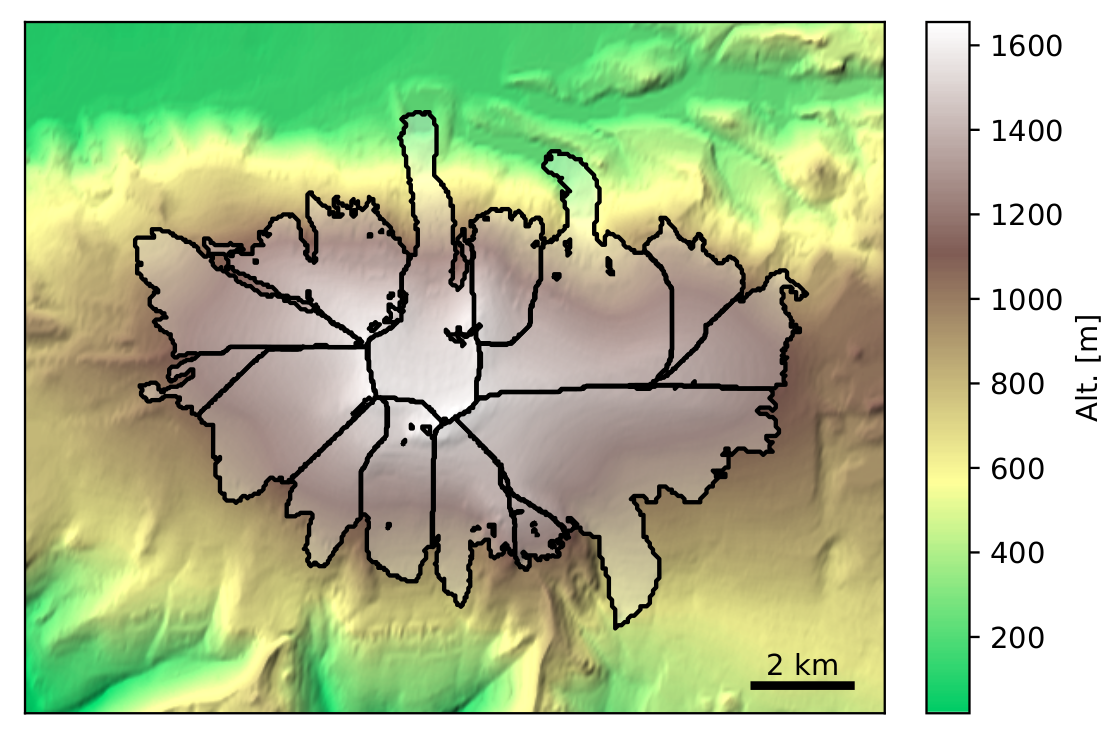
\includegraphics[width=0.7\linewidth]{\figs/iceland.png}
\caption{Glacier centric approach applied to the Eyjafjallajökull ice cap in Iceland.  Glacier outlines provided by the Randolph Glacier Inventory v6.0.}
\end{figure}

The glacier centric approach is used by most large-scale glacier models to date. Alternative strategies include global
gridded approaches \citep{Shannon2019}, where all glaciers in a model grid cell are added together and possibly
organized into elevation bins. Another approach is to handle entire glacier complexes as one single body of ice (“ice
caps”). This is physically consistent and feasible, but requires either distributed models of ice flow
\citep{Furst2017} (computationally expensive) or implies simplifications to the glacier geometry (so that all ice flows
downwards, \citep{Huss2012}).

The advantage of glacier centric models is their adherence to the de-facto standard inventory of glacier outlines:
the \href{https://www.glims.org/RGI/}{Randolph Glacier Inventory}. Any glacier can be selected and simulated, and the model
output can be compared to standard reference datasets such as length changes or surface mass balance data from
the \href{https://wgms.ch}{World Glacier Monitoring Service}. Various models can be compared on a glacier per glacier basis
or a combination of them. It is also computationally efficient, since models can focus on simulating the areas where
glaciers are really located. This may sound trivial, but glacier centric models can also make use of the glacier
location as a boundary condition, e.g. by excluding unrealistic solutions to the problem of computing mass balance or
inferring ice thickness, for example.

The disadvantage of glacier centric models is their questionable scientific validity in presence of glacier complexes
and ice divides (this problem can be mitigated by defining glacier complexes as one single entity, requiring other
strategies than currently standard in OGGM). A larger issue of glacier centric models is that they are focussed on
simulating glaciers that have been inventoried, i.e. they cannot retrieve past (or present) uncharted glaciers
\citep{Parkes2018}. For these reasons, they are not well adapted for studying glacier evolution in climates when
glaciers were widely different from today (e.g. the Last Glacial Maximum).


\subsection{Standard modelling workflow}

I briefly illustrate the OGGM workflow with an example application on the Tasman Glacier in New Zealand (see figure
below). Refer to the model documentation for more information.

\textbf{Preprocessing.}
The glacier outlines are extracted from a reference dataset (RGI)
and projected onto a local gridded map of the glacier (Fig.~\ref{fig:flow}a). Depending on the glacier location, a suitable source
for the topographical data is downloaded automatically and interpolated to the local grid. The spatial resolution of the
map depends on the size of the glacier.

\textbf{Flowlines.}
The glacier centerlines are computed using a geometrical routing algorithm
(Fig.~\ref{fig:flow}b), then filtered and slightly modified to become glacier “flowlines”
with a fixed grid spacing (Fig.~\ref{fig:flow}c).

\textbf{Catchment areas and widths.}
The geometrical widths along the flowlines are obtained by intersecting the normals at each grid point with the glacier
outlines and the tributaries’ catchment areas. Each tributary and the main flowline has a catchment area, which is then
used to correct the geometrical widths so that the flowline representation of the glacier is in close accordance with
the actual altitude-area distribution of the glacier (Fig.~\ref{fig:flow}d).

\textbf{Climate data and mass balance.}
Gridded climate data (monthly temperature and precipitation) are interpolated to the glacier location and corrected for
the altitude at each flowline’s grid point. A calibrated mass balance model is used to compute the mass balance for the
past, and for projections based on GCM data.

\textbf{Ice thickness inversion.}
Using the mass balance data computed above and relying on mass-conservation considerations, an estimate of the ice flux
along each glacier grid point cross-section is computed by making assumptions about the shape of the cross-section.
Using the physics of ice flow and the shallow ice approximation, the model then computes the thickness of the glacier
along the flowlines and the total volume of the glacier (Fig.~\ref{fig:flow}e).

\textbf{Glacier evolution.}
A dynamical flowline model is used to simulate the advance and retreat of the glacier under preselected climate time
series. Here (Fig.~\ref{fig:flow}f), a 120-yrs long random climate sequence leads to a glacier advance.


\begin{figure}[h]
\centering
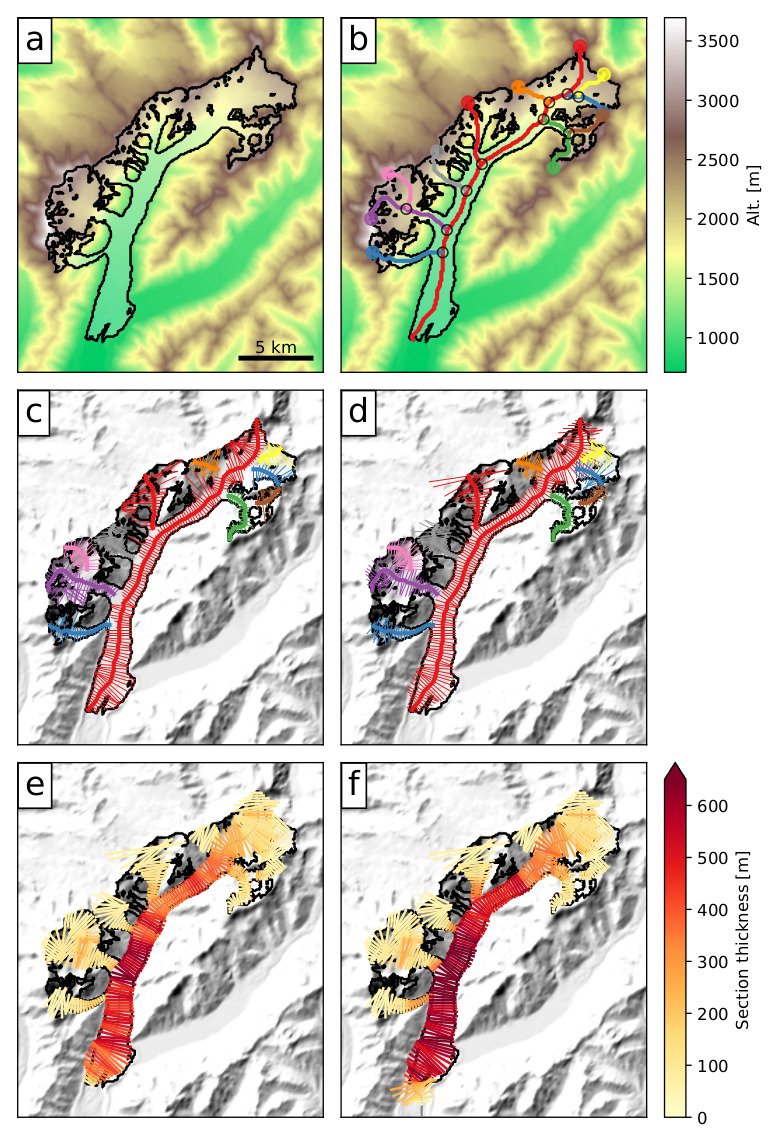
\includegraphics[width=0.700\linewidth]{\figs/ex_workflow.png}
\caption{Illustration of the OGGM standard workflow applied to Tasman Glacier.}
\label{fig:flow}
\end{figure}


\subsection{OGGM data structures and glacier directories}

The fundamental data structure used in OGGM is the so-called \textbf{Glacier Directory}. Glacier directories simply are
folders on disk which store the input and output data for a single glacier during a run. OGGM offers an object interface
to access and store these files programmatically.

This very simple idea is at the core of the OGGM workflow: actions to perform on glaciers (“tasks”, see below) are given
access to the data files via the glacier directory interface, read data they need from disk, and write back to it.

This design matches perfectly the “glacier centric” modelling strategy, and has many advantages:
\begin{itemize}
\item {} 
there is no practical difference between simulating one single, or many glaciers: all glacier directories are
independent of another.

\item {} 
data is persistent on disk: workflows can be interrupted and restarted from disk at no cost overhead. Workflows can
even be prepared on one computer and restarted from another computer (see example below).

\item {} 
“modularity” is achieved via data formats, not via programmatic interfaces: various ways to compute the flowlines (for
example) can co-exist if they agree on how a flowline is stored on disk.

\item {} 
multiprocessing is trivial: the same task can be run on many glaciers at once without having to share data across
processes, since everything is on disk and independant.

\end{itemize}

This persistence en disk has a few drawbacks as well:
\begin{itemize}
\item {} 
for the glacier directories to be independent, several data sources are duplicated: topography for example (each
glacier has its own subset of the original data, often overlapping with neighbors), or climate timeseries (the same
data from the same grid point is stored in various directories). This can lead to rather large data storage
requirements, but can be mitigated by deleting intermediate files.

\item {} 
since users can restart workflows from pre-processed states, the code that was used to produce them is often ignored
or might be older, etc. This can lead to silent bugs (for example mismatching model parameters between the preprocessing
and the simulations, leading to incorrect results). Because of this issue, we had to implement safeguards against such
mistakes where possible.

\item {} 
users can be confused by glacier directories. Since an OGGM program does not always read like linear “A to Z”
workflows (but for example “start from Q, then Q to Z”), mistakes like the ones described above can happen unnoticed.

\item {} 
it can make certain types of sensitivity experiments more difficult to implement, since users not only have to care
about variable names, but also data file names.

\end{itemize}

Here is an example of how glacier directories work in practice. The user indicates a repository from which
they want to fetch the data, and a list of glacier IDs they’d like to start from. The \mintinline{python}{init_glacier_directories}
performs the action of downloading and extracting these data locally.

\begin{figure}[H]
\captionsetup{singlelinecheck = false, justification=justified} 
\begin{minted}
[
]
{python}
from oggm import workflow, graphics

# Glaciers to simulate
rgi_ids = ['RGI60-11.01328', 'RGI60-11.00897']
# Where to fetch the pre-processed directories - this can be changed
server_url = 'https://cluster.klima.uni-bremen.de/~oggm/gdirs/'
experiment_url = 'oggm_v1.4/L3-L5_files/CRU/centerlines/qc3/pcp2.5/no_match'
base_url = server_url + experiment_url
# Fetch them
gdirs = workflow.init_glacier_directories(rgi_ids, from_prepro_level=3, 
                                          prepro_base_url=base_url)
# Plot the ice thickness inversion results
graphics.plot_inversion(gdirs[0])
\end{minted}
\vspace{10mm}
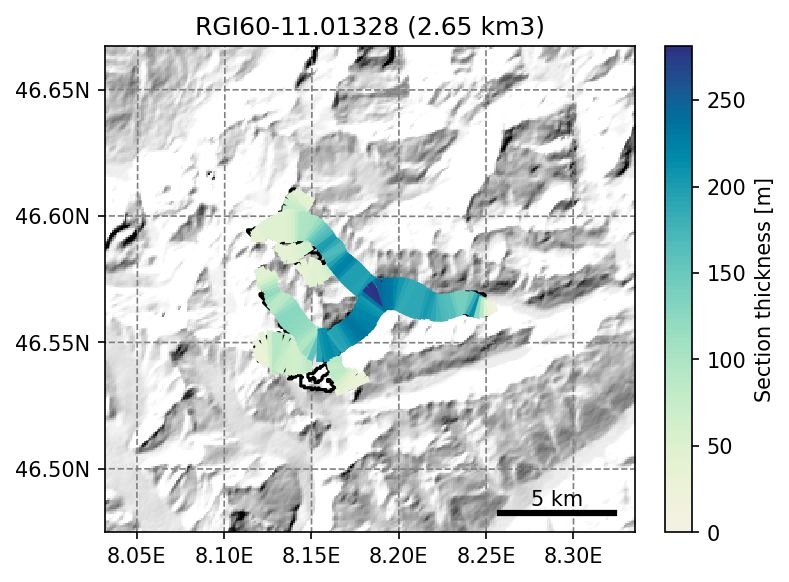
\includegraphics[width=0.600\linewidth]{\figs/unteraar_demo.png}
\caption{Example of the glacier directory workflow}
\end{figure}

See also the documentation page for \href{https://docs.oggm.org/en/stable/input-data.html}{OGGM-Shop}
for more examples of the kind of data that can be added to glacier directories.


\subsection{OGGM tasks}

Tasks in OGGM are actions to perform on one single glacier (“entity tasks”) or several of them (“global tasks”). Tasks
have a special meaning in the OGGM workflow and are applied as such:

\begin{figure}[H]
\begin{minted}
[
]
{python}
# Initialize glacier dir
from oggm import workflow, tasks

ectories
gdirs = workflow.init_glacier_directories(rgi_ids)

# Define the list of tasks
task_list = [
    tasks.define_glacier_region,
    tasks.glacier_masks,
    tasks.compute_centerlines,
    tasks.catchment_area,
    tasks.catchment_width_geom,
]

# Apply them sequentially
for task in task_list:
    workflow.execute_entity_task(task, gdirs)
\end{minted}
\end{figure}


\mintinline{python}{exectute_entity_task} will apply the given task to a list of glaciers. If multiprocessing is switched on, all glaciers
will be processed in parallel, making full use of all available processors. Here we apply the default tasks with default
settings, but parameters can be changed via global settings or function arguments.

Depending on the desired set-up, tasks can be replaced by others (e.g. the centerlines tasks can be replaced by other
algorithms) or omitted (for example, users can choose whether a quality check filter should be applied to the climate
timeseries or not).


\begin{figure}[h]
\centering
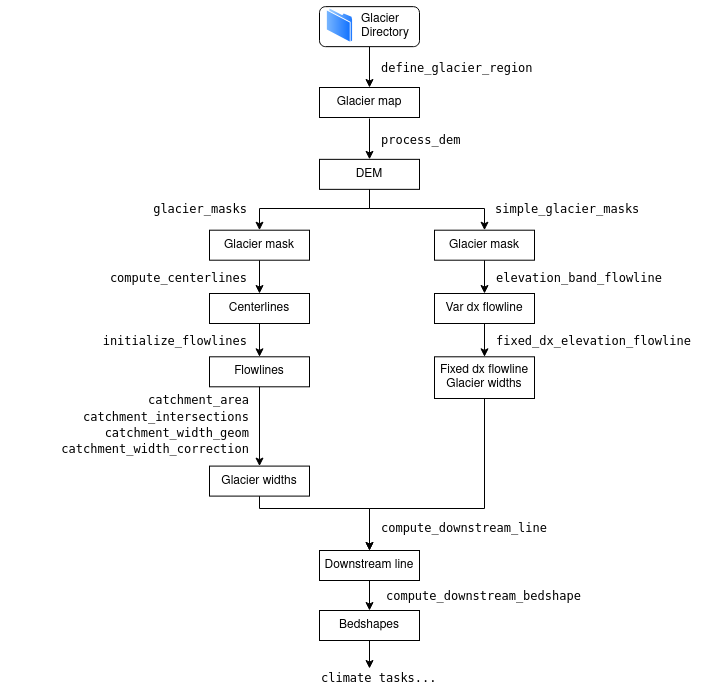
\includegraphics[width=0.700\linewidth]{\figs/flowchart_flowlines.png}
\caption{Example flowchart illustrating how OGGM implemented support for two kinds
of flowline representations for a glacier: centerlines on the left (OGGM’s default)
and binned elevation bands flowlines on the right (after \citet{Huss2012}).}
\end{figure}

\subsection{Take home messages}

The purpose of this rather technical description was to convey the general design of the model around the concept of a
list of tasks to be applied to glacier entities and that store their output in glacier directories on disk. Note that
except for their names and the objects they are referring to (glaciers), these “building blocks” are largely
agnostic to the kind of tasks that have to be applied, and I deliberately did not provide any modelling detail here.

This is important, because I believe that the OGGM project should not be considered by looking only at the physics
choices we’ve made for each of these tasks or their default parameters. OGGM should also be evaluated for the new
developments its structure can allow. OGGM does not enforce a particular modelling strategy beyond the constraints
defined above: in summary, complying models do need to follow the glacier directory approach (otherwise OGGM will be of
very little use for them). If new modelling groups develop ideas based on a glacier centric approach, they can make use
of OGGM’s building blocks and add their own, provided that they comply with this “OGGM way of doing things”.

By doing so, external projects based on OGGM will then benefit from all future developments in OGGM, and the other way
around: OGGM can then use and apply these external modules. If desired, external projects can also benefit from the
suite of modern open development tools that OGGM provides. I describe them below.


\section{Open development practices}

OGGM development has been strongly inspired by practices which have become a standard in the software development
community, but that are (unfortunately) not yet well known in the scientific community.

Like the vast majority of today’s software, OGGM’s development is done under a version control system
called \href{https://git-scm.com/}{git}. The OGGM repository is hosted on \href{https://github.com/OGGM/oggm}{github}, enabling
many of the tools described below.


\subsection{Code review}

Very much like peer-review, open development practices based on git enable code review. Open code review has many
advantages:
\begin{itemize}
\item {} 
it gives model developers the opportunity to discuss changes alongside the code rather than per email

\item {} 
it improves code quality, since more than one person can look at the code

\item {} 
it gives an opportunity to model users to follow changes in the model even if they are not actively participating

\item {} 
code changes and associated comments over time are stored online for later reference

\end{itemize}


\begin{figure}[h]
\centering
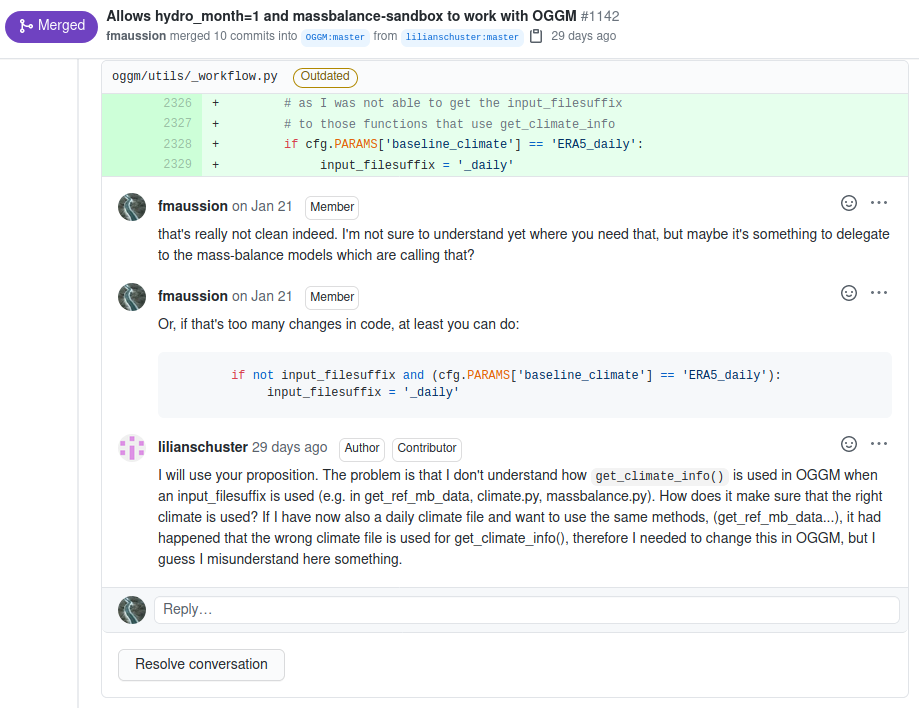
\includegraphics[width=0.900\linewidth]{\figs/pr.png}
\caption{Example of code review in a recent “\href{https://github.com/OGGM/oggm/pull/1142}{pull-request}”.}
\end{figure}

Ideally, all code submissions to OGGM should be peer-reviewed. In practice, however, only the contributions from others
than me are reviewed (by me). I’ll discuss this problem in more length below.


\subsection{Testing strategy}

OGGM enforces a strict code testing strategy: all additions to the code must be supplemented by appropriate tests. The
tests have the purpose to check that the code (i) can be executed without errors and (ii) works as expected. These tests
are an integral part of the codebase, and all of them are run each time a new code addition is suggested (a process
called \href{https://en.wikipedia.org/wiki/Continuous\_integration\#Run\_tests\_in\_CI}{continuous integration}), hereby
avoiding “regressions” as much as possible (when a change in one part of the code affects another in non-predictable
ways).

\begin{figure}[h]
\centering
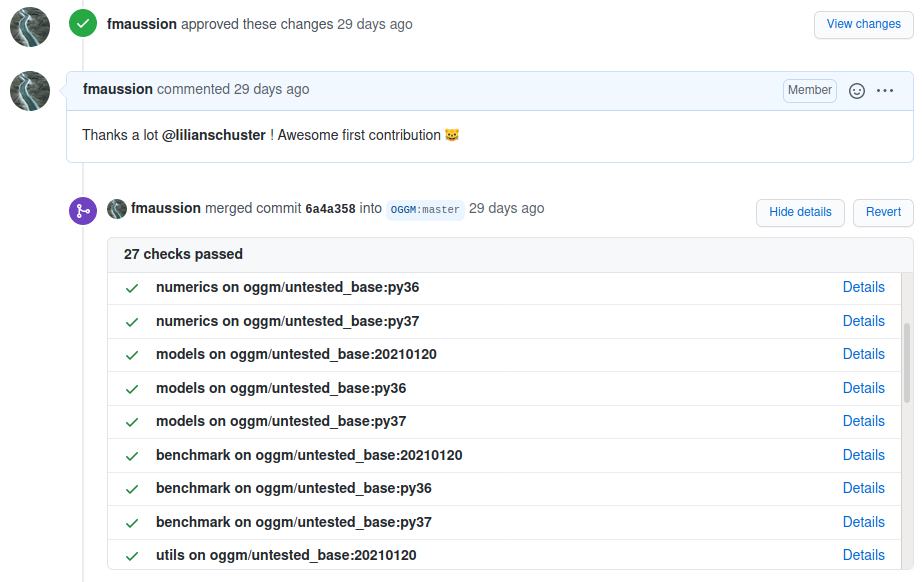
\includegraphics[width=0.700\linewidth]{\figs/tests.png}
\caption{Example of automated testing in a recent “\href{https://github.com/OGGM/oggm/pull/1142}{pull-request}”.}
\end{figure}


\subsection{Online documentation and tutorials}

Making code available is, by far, not enough to make code accessible. As of today, the OGGM codebase contains several
thousands of lines of code, making it very difficult for anyone new to the project to understand the model’s structure
just by reading the code.

Lack of code documentation (and the high cost of writing documentation) is probably one of the main obstacles towards
more open code sharing practices, as many scientists do not feel comfortable to share undocumented code. OGGM is no
exception (I always feel there could be better documentation for almost everything), but thanks to a suite of great
open-source tools, writing documentation for OGGM can also be rewarding. Writing documentation is also a very good way
to engage the community of users towards OGGM’s development, since contributing to the documentation can feel easier
than contributing to the code.

OGGM’s documentation relies on three main elements:
\begin{enumerate}

\item {} 
The project website (\href{https://oggm.org}{https://oggm.org}) for general, non code related project communication and blog posts.

\item {} 
The technical documentation (\href{https://docs.oggm.org}{https://docs.oggm.org}) to document model physics, model structure, and function calls
definitions.

\item {} 
The tutorials (\href{https://oggm.org/tutorials}{https://oggm.org/tutorials}) with hands-on model applications in various use cases.

\end{enumerate}

The project website is built using \href{https://jekyllrb.com/}{jekyll}, a static site generator. It’s source code and
content is also open and stored \href{https://github.com/OGGM/oggm.github.io}{on github}.

The technical documentation is built using \href{https://www.sphinx-doc.org}{sphinx} and is hosted
on \href{https://readthedocs.org/}{readthedocs}. Its content is stored alongside the code on the main repository.

The tutorials are written with \href{https://en.wikipedia.org/wiki/Project\_Jupyter\#Jupyter\_Notebook}{Jupyter Notebooks} and
rendered online with \href{https://jupyterbook.org}{Jupyter-Book}. The notebook interface allows sharing text and formulas
alongside the code, making them particularly adapted for tutorials. In addition, tutorials can be run and explored
interactively thanks to \href{https://mybinder.org}{MyBinder}. This is a great tool to engage new users, since they can try
the model online before going the struggle of installing it.


\subsection{Reproducibility}

OGGM attempts to make results obtained with the
model \href{https://en.wikipedia.org/wiki/Reproducibility\#Reproducible\_research}{reproducible} as far as possible. To do so,
the OGGM stable versions are stored with a DOI on \href{https://zenodo.org/record/4546676}{Zenodo}, and authors
are \href{https://docs.oggm.org/en/stable/citing-oggm.html}{encouraged} to use and cite stable OGGM versions (we can also
store older versions on demand if necessary).

Furthermore, a central tool that we offer to ensure that OGGM results are reproducible no matter the machine it is
running on, or the version of software packages that are installed
are \href{https://docs.oggm.org/en/stable/practicalities.html\#singularity-and-docker-containers}{docker containers}.
Containers are like a “software capsule”: they contain everything that OGGM needs to run and can be executed by any
machine that has Docker installed.


\section{Challenges}

To my knowledge at the time of writing, OGGM has been used for at least 13 peer-reviewed publications (3 are in review)
and has been an important part of 3 completed PhD theses. We expect these numbers to grow in the future, with new
generations of students and new collaborations starting just now. Several other indicators are suggesting that the OGGM project is being used by other
research groups, such as the number of requests to join our discussion channels and to use OGGM-Hub.

The fact that the OGGM project is now expected to suit these various needs
(new users with various expectations about OGGM capabilities, PhD students and PostDocs under time pressure,
project deadlines, etc) comes with a number of challenges which I briefly describe here.


\subsection{Technical debt}

The OGGM code base has grown and continues to grow organically, at the pace at which new features are added to the
model. Future innovation will be slowed down and maybe even impeded by the so-called “technical debt”: code that works
but would need considerable refactoring to adapt to new ideas and to allow further development.

Accumulating technical debt also makes testing the software and ensuring the validity of its results more challenging.
Certain functions might have been written in the past to take into account situations which are no longer an issue
today, adding unnecessary complexity to the code.

This often needed refactoring (process of restructuring and modernizing existing computer code)
is not without costs: it takes considerable time, is not rewarded by traditional academic measures such as publications,
and needs to be carefully conducted in order not to introduce new bugs into the software. Perhaps even more
problematically: existing users who wrote code based on OGGM are very unwilling to update it to the new OGGM versions (I
know this from experience).

There is therefore a trade-off between breaking backwards compatibility (i.e. breaking existing code) and
innovating. Other models with fewer users, or lower standards in terms of code reusability (this is not always a bad thing),
may be more agile and quicker in innovating because no other people are relying on their code being stable.


\subsection{Software maintenance and entry level for new contributors}

A large part of routine software development maintenance currently relies on one or two main developers (myself, and an
IT technician in Bremen who is in charge of the technical aspects of the deployment of OGGM).
This work takes a lot of time (mainly because every new feature needs to be tested and documented), and my time is
limited. Therefore, the development process is slower than I’d like it to be.

As the software grows and increases in complexity, it becomes more difficult for new users to understand the model’s
structure and to apply it to their specific research problem. Furthermore, it makes it harder for new users to
envision a potential contribution to the code base. The typical model contributors (PhD students and post docs) are
employed on fixed-term contracts, causing a high turnover, making transmission of knowledge particularly difficult.

Finally, not all scientists are interested in writing reusable code, as is required when contributing to OGGM.
Very few have the time, energy, or interest to invest in the rather demanding field of scientific programming,
while staying on top of the other requirements of our job. I had the privilege to be given enough time to realize this
project over the course of several years, thanks to my stable employment at the university of Innsbruck. No other
traditional funding scheme in Austria would have allowed this kind of long haul development work.

The future of OGGM’s technical development and maintenance therefore strongly relies on funding agencies
acknowledging that open-source development work is an integral part of the scientific process. Employers should reward
open source work at the same level as scientific publications when considering applications.


\subsection{Innovation with OGGM}

I often ask myself the question of the role of OGGM in comparison to similar models in the geosciences.
Let’s take the atmospheric model \href{https://www.mmm.ucar.edu/weather-research-and-forecasting-model}{WRF}
as a prominent example. WRF is open-source, and its user base is obviously larger than OGGM by several orders of
magnitude. The reason is not only that WRF is an atmospheric model, and a much more mature and feature complete model.
I believe that a major reason is that users can take the model, learn how to use it (without knowing the internal
details of its functioning), and apply it to their research question with very few modifications (change of domain,
change of boundary conditions).

Attempting to make a parallel with OGGM will unravel some differences:

\begin{itemize}
\item {} 
For one, OGGM already simulates
all glaciers. I.e. “changing the domain” is not meaningful, unless the study attempts to simulate glaciers
differently, or analyse the data from a new perspective.

\item {} 
Second, since OGGM is highly parameterized, applying it blindly, without a specific awareness of its simplifications
and potential pitfalls, is not recommended.
This point is also valid for WRF, but I would argue that it is less problematic: thanks to the large
amount of available data for independent validation, users are able to check if their simulations are meaningful.
With a model like WRF, where the boundaries between calibration and validation data are fuzzier, it is difficult
for users to assess whether they apply the model correctly or not.

\item {} 
Finally, application of OGGM to a new research question almost inevitably leads to the development of extensions to
OGGM, or modifications of its internal code. This comes with the nature of the model: since the standard modelling of all
glaciers is possible “out-of-the box”, innovation can only come with active participation in the model development,
it’s capacity to deal with new boundary conditions, a new model parameterization, etc.

\end{itemize}

To summarize, and despite all our efforts to make OGGM user-friendly, I think that for the time being OGGM is
still a model “for modellers”, not yet ready for blind application. Because of the nature of the problems that
OGGM is trying to solve, it might never be “a model for users”, and remain “a model (or framework) for modellers”.
I think that this is something I’d be happy with, but it has implications for the people willing to learn how to apply
the model -- in particular in terms of required programming and glacier modelling skills.
\cleardoublepage

\newcommand{\papertext}{Paper 01: Model description}

\section*{\papertext}
\addcontentsline{toc}{section}{\protect\numberline{}\papertext}%
\label{paper_01}

\vspace{0.5cm}

\begin{singlespace}
\begin{hangparas}{1em}{1}
\textbf{Maussion, F.}, Butenko, A., Champollion, N., Dusch, M., Eis, J., Fourteau, K., Gregor, P., Jarosch, A. H., Landmann, J., Oesterle, F., Recinos, B., Rothenpieler, T., Vlug, A., Wild, C. T. and Marzeion, B.: The Open Global Glacier Model (OGGM) v1.1, Geosci. Model Dev., 12(3), 909–931, \\
\href{https://doi.org/10.5194/gmd-12-909-2019}{doi:10.5194/gmd-12-909-2019}, 2019.
\end{hangparas}
\end{singlespace}

\vspace{0.5cm}


%\includepdf[pages=-,openright]{./papers/paper_01.pdf}



\chapter{Ice thickness estimation}
\label{chap3}

\cleardoublepage

\renewcommand{\papertext}{Paper 02: How accurate are estimates of glacier ice thickness? Results from ITMIX, the Ice Thickness Models Intercomparison eXperiment}

\section*{\papertext}
\addcontentsline{toc}{section}{\protect\numberline{}\papertext}%
\label{paper_02}

\vspace{0.5cm}

\begin{singlespace}
\begin{hangparas}{1em}{1}
Farinotti, D., Brinkerhoff, D. J., Clarke, G. K. C., Fürst, J. J., Frey, H., Gantayat, P., Gillet-Chaulet, F., Girard, C., Huss, M., Leclercq, P. W., Linsbauer, A., Machguth, H., Martin, C., \textbf{Maussion, F.}, Morlighem, M., Mosbeux, C., Pandit, A., Portmann, A., Rabatel, A., Ramsankaran, R., Reerink, T. J., Sanchez, O., Stentoft, P. A., Singh Kumari, S., van Pelt, W. J. J., Anderson, B., Benham, T., Binder, D., Dowdeswell, J. A., Fischer, A., Helfricht, K., Kutuzov, S., Lavrentiev, I., McNabb, R., Gudmundsson, G. H., Li, H. and Andreassen, L. M.: How accurate are estimates of glacier ice thickness? Results from ITMIX, the Ice Thickness Models Intercomparison eXperiment, Cryosph., 11(2), 949--970, \href{https://doi.org/10.5194/tc-11-949-2017}{doi:10.5194/tc-11-949-2017}, 2017.
\end{hangparas}
\end{singlespace}

\vspace{0.5cm}

This paper is the result of an international working group of the International Association of
Cryospheric Sciences (IACS): the working group on \href{https://cryosphericsciences.org/activities/ice-thickness}{Glacier ice thickness estimation}  (2014--2019),
of which I was a member. The group activities led to several major publications, two of them are presented in
this thesis.

The first collaborative effort of the working group was the “Ice Thickness Models Intercomparison eXperiment (ITMIX)”,
phase 1. It was the first coordinated assessment of the individual performance of independent methods able to infer
glacier ice thickness from characteristics of the surface. A set of 17 different models were used to estimate the ice
thickness “blindly”, i.e. without using any observations for model calibration or tuning.

This publication is a milestone in the field of glacier ice thickness estimation. Cited more than 110 times to date (
Google Scholar), it laid the ground for a wealth of follow-up studies, leading several research groups (including mine)
to increase efforts in developing new methods to estimate the volume of glaciers. Indeed, we showed that the
disagreement between models themselves and between models and observations can be very large (up to several times the
observed ice thickness). Ensemble approaches may reduce model errors, but no model consistently outperformed the others.
A few models were favorably listed for their ability to robustly simulate many glaciers with a reasonable accuracy (e.g.
OGGM, Huss), or for their high accuracy on fewer glaciers (e.g. Brinkerhoff-v1),

My contribution to this paper was the participation in several meetings that helped to shape the experimental design,
and I participated with a model contribution. OGGM was ranked among the best models able to estimate ice thickness from
limited information (i.e. able to compute many glaciers). I also contributed to the analysis of the
results, and played a minor role in the writing of the paper.


\href{https://doi.org/10.5194/tc-11-949-2017}{Link to the paper} (open access).


%\includepdf[pages=-,openright]{./papers/paper_02.pdf}


\cleardoublepage

\renewcommand{\papertext}{Paper 03: A consensus estimate for the ice thickness distribution of all glaciers on Earth}

\section*{\papertext}
\addcontentsline{toc}{section}{\protect\numberline{}\papertext}%
\label{paper_03}

\vspace{0.5cm}

\begin{singlespace}
\begin{hangparas}{1em}{1}

Farinotti, D., Huss, M., Fürst, J. J., Landmann, J., Machguth, H., \textbf{Maussion, F.} and Pandit, A.: A consensus estimate for the ice thickness distribution of all glaciers on Earth, Nat. Geosci., 12(3), 168--173, \href{https://doi.org/10.1038/s41561-019-0300-3}{doi:10.1038/s41561-019-0300-3}, 2019.

\end{hangparas}
\end{singlespace}

\vspace{0.5cm}


This paper is the second contribution of the IACS working group on Ice thickness estimation. After the completion of
ITMIX experiment phase I, all modelling groups able to simulate many glaciers (\textgreater{} 1000)
were invited to contribute to the first global, multi-model estimate of the distributed ice thickness of the
world’s glaciers. This was a very timely endeavor, for various reasons:
\begin{itemize}[nosep]
\item {} 
the only previous global estimate of distributed glacier ice thickness \citep{Huss2012} was based on a single model
and on an older version of the RGI glacier inventory

\item {} 
other glacier volume estimates (i.e. without distributed thickness) were based on scaling relationships, and were
widely different from another \citep{Radic2010,Marzeion2012,Grinsted2013}

\item {} 
there was an increasing demand from the community for a freely available, RGI based ice thickness product.

\end{itemize}

Similarly to ITMIX phase I, the call for participation was open to anyone, and the boundary conditions (topography, ice
thickness observations) were standardized and provided to all participants. Importantly, the modellers were asked to
conduct a cross-validation experiment, in which the training and validation samples were rotated to allow an independent
model validation. The final weight given to each model contribution would depend on its out-of-sample validation score.

The main outcome of this study certainly is the openly available ice-thickness dataset, which is now advertised as an
extended product of the RGI version 6. Similarly to ITMIX phase I, the study also reveals large discrepancies between
models, indicating that further improvements will be necessary (I will discuss this point
in Sect.~\ref{perspectives}).

I contributed to this paper in several ways. OGGM was one of the five models contributing to the final product. 
I argued in favor of running a cross-validation experiment and helped designing it. I also participated with an 
additional model contribution (a simple statistical model), which was later discarded because it was previously unpublished.
I participated in the analysis of the results, and, to a smaller extent, to the writing of the paper.

\href{https://doi.org/10.1038/s41561-019-0300-3}{Link to the paper} (non open-access) \\
\href{https://doi.org/10.3929/ethz-b-000315707}{Link to the ice thickness dataset} (open-access)

\iflong \includepdf[pages=-,openright]{./papers/paper_03.pdf} \else \fi 


\cleardoublepage

\renewcommand{\papertext}{Paper 04: Impact of frontal ablation on the ice thickness estimation of marine-terminating glaciers in Alaska}

\section*{\papertext}
\addcontentsline{toc}{section}{\protect\numberline{}\papertext}%
\label{paper_04}

\vspace{0.5cm}

\begin{singlespace}
\begin{hangparas}{1em}{1}

Recinos, B., \textbf{Maussion, F.}, Rothenpieler, T. and Marzeion, B.: Impact of frontal ablation on the ice thickness estimation of marine-terminating glaciers in Alaska, Cryosph., 13(10), 2657--2672, \href{https://doi.org/10.5194/tc-13-2657-2019}{doi:10.5194/tc-13-2657-2019}, 2019.

\end{hangparas}
\end{singlespace}

\vspace{0.5cm}

This paper is the first of two papers led by Beatriz Recinos during her PhD
Thesis at the University of Bremen (\href{https://media.suub.uni-bremen.de/handle/elib/4637}{link to the PDF}). In this work, we studied the influence of
frontal ablation on the OGGM ice thickness estimation of marine-terminating glaciers.

OGGM’s ice thickness model belongs to the type of “mass-conservation models”, which rely on the computation of an ice
flux through the glacier. Using this flux value, surface properties and the physics of ice flow, OGGM estimates the ice
thickness along the flowline. In this paper, we discuss (for the first time in a regional modelling context) the
importance of frontal ablation on the estimation of this mass flux and therefore on the volume of marine-terminating
glaciers.

We implemented an existing parameterization \citep{Oerlemans2005b} in OGGM to estimate frontal ablation flux from three
simple variables (ice thickness, water depth, and glacier width) and one tuning parameter. Relying on the assumption
that this flux needs to be equal to the flux by ice deformation at the terminus, we could solve for the ice thickness at
the terminus and provide this new boundary condition to the mass balance model calibration routine.

This publication led to the operational implementation of this parameterization in OGGM, and paved the way for further
investigation. While we still relied on an external frontal ablation dataset to calibrate model parameters, in a
follow-up study (Recinos et al., in review for J. Glac.), we could make use of observations of ice velocity to better
calibrate the model.

I contributed to this paper in several ways: I provided technical support to Beatriz in the implementation of the new
parameterization, and I helped with the OGGM integration. I also provided support and supervision during the paper
writing and during the review process.

\href{https://doi.org/10.5194/tc-13-2657-2019}{Link to the paper} (open access)


%\includepdf[pages=-,openright]{./papers/paper_04.pdf}


\cleardoublepage

\renewcommand{\papertext}{Paper 05: Bias-corrected estimates of glacier thickness in the Columbia River Basin, Canada}

\section*{\papertext}
\addcontentsline{toc}{section}{\protect\numberline{}\papertext}%
\label{paper_05}

\vspace{0.5cm}

\begin{singlespace}
\begin{hangparas}{1em}{1}

Pelto, B. M., \textbf{Maussion, F.}, Menounos, B., Radić, V. and Zeuner, M.: Bias-corrected estimates of glacier thickness in the Columbia River Basin, Canada, J. Glaciol., 1--13, \href{https://doi.org/10.1017/jog.2020.75}{doi:10.1017/jog.2020.75}, 2020.

\end{hangparas}
\end{singlespace}

\vspace{0.5cm}

Ben Pelto approached me when he was working on his doctoral thesis about glaciers in the Columbia and Rocky Mountains,
Canada
(\href{https://unbc.arcabc.ca/islandora/object/unbc\%3A59097?solr\_nav\%5Bid\%5D=551a2e3c2ca38d6ce42a\&solr\_nav\%5Bpage\%5D=0\&solr\_nav\%5Boffset\%5D=1}{link to the thesis}).
His goal was to use OGGM to compute glacier thickness in the Columbia River Basin, using newly acquired ice thickness
and mass balance measurements.

While there exists a volume estimate for every glacier in the world (Paper 03), they can be subject to large
uncertainties at the single glacier or catchment scale. Using ground penetrating radar (GPR) observation campaigns, Ben
Pelto and colleagues found that the 2019 consensus ice thickness estimates were consistently too low for this catchment.

This study is a good example of the kind of collaboration that the OGGM project was designed for: using established
methods but adding value with new observational data, expert knowledge and an improved calibration scheme, we were able
to reduce model uncertainties and provide more accurate estimates of ice thickness in the region. The paper received
some local media attention after publication, which will surely benefit Ben Pelto’s career development.

I contributed to this paper by providing technical support with OGGM, as well as helping designing the calibration and
validation strategy, which involved using cross-validation to better estimate the out-of-sample accuracy of the model. I
also played a minor role in the writing of the paper.

\href{https://doi.org/10.1017/jog.2020.75}{Link to the paper} (open-access)


\iflong \includepdf[pages=-,openright]{./papers/paper_05.pdf} \else \fi 



\chapter{Glacier mass balance}
\label{chap4}

\cleardoublepage

\renewcommand{\papertext}{Paper 06: ENSO influence on surface energy and mass balance at Shallap Glacier, Cordillera Blanca, Peru}

\section*{\papertext}
\addcontentsline{toc}{section}{\protect\numberline{}\papertext}%
\label{paper_06}

\vspace{0.5cm}

\begin{singlespace}
\begin{hangparas}{1em}{1}

\textbf{Maussion, F.}, Gurgiser, W., Großhauser, M., Kaser, G. and Marzeion, B.: ENSO influence on surface energy and
mass balance at Shallap Glacier, Cordillera Blanca, Peru, Cryosph., 9(4), 1663--1683,
\href{https://doi.org/10.5194/tc-9-1663-2015}{doi:10.5194/tc-9-1663-2015}, 2015.

\end{hangparas}
\end{singlespace}

\vspace{0.5cm}

This study was conducted during my first PostDoc assignment at the University of Innsbruck, within the project
“Multidecadal to Centennial Climate Variability: Assessing the Conditions for the Glaciation of Tropical Mountains”.
Based on a 4-year long time series of distributed surface energy and mass balance (SEB/SMB, calculated using a
process-based model driven by observations), we developed a statistical model able to predict (downscale) monthly
SEB/SMB components from large-scale atmospheric reanalysis data. We then used these 34-yrs long reconstructions to study
the impact of ENSO on SEB and SMB fluxes at Shallap Glacier, Cordillera Blanca, Peru.

This paper also led to the publication of an open-source package written in
Python (\href{https://bitbucket.org/fmaussion/downglacier}{DownGlacier}). I could then apply some of the practices I
learned during the writing of this software to OGGM, which was only a vague project idea at that time. More importantly, this
study contributed to the growing literature and interest for the application of machine learning techniques in
glaciology. An important follow-up project (unrelated to me) is the \href{https://github.com/JordiBolibar/ALPGM}{ALPGM} model
\citep{Bolibar2020}, developed by Jordi Bolibar at the University of Grenoble.

My contribution to this paper was the development of the downscaling method, the generation of the figures and the
writing of the paper.

\href{https://doi.org/10.5194/tc-9-1663-2015}{Link to the paper} (open-access) \\
\href{https://bitbucket.org/fmaussion/downglacier}{Link to the open software “DownGlacier”}


\iflong \includepdf[pages=-,openright]{./papers/paper_06.pdf} \else \fi 


\cleardoublepage

\renewcommand{\papertext}{Paper 07: Robust uncertainty assessment of the spatio-temporal transferability of glacier mass and energy balance models}

\section*{\papertext}
\addcontentsline{toc}{section}{\protect\numberline{}\papertext}%
\label{paper_07}

\vspace{0.5cm}

\begin{singlespace}
\begin{hangparas}{1em}{1}

Zolles, T., \textbf{Maussion, F.}, Galos, S. P., Gurgiser, W. and Nicholson, L.: Robust uncertainty assessment of the spatio-temporal transferability of glacier mass and energy balance models, Cryosph., 13(2), 469--489, \href{https://doi.org/10.5194/tc-13-469-2019}{doi:10.5194/tc-13-469-2019}, 2019.

\end{hangparas}
\end{singlespace}

\vspace{0.5cm}

This study is the outcome of a master thesis that Tobias Zolles wrote under my supervision. The original idea came
during a “paper club” were we discussed an interesting paper by Rye and co-authors \citep{Rye2012}. In their study, the
authors argued for the use of “multiobjective optimization” in glacier mass balance models to reduce model uncertainty.
While we agreed with the main premise of the paper, we also noted that the main argument (that a model calibrated on more
than one observable variable was more accurate) was based on a validation procedure realized on the same dataset
as the one used for calibration. We therefore decided to apply multiobjective calibration in a new setting:
with a full SEB/SMB model, and using
cross-validation to assess the value of the calibration with data unseen by the model. In addition, we conducted an
extensive sensitivity analysis to reduce the parameter space before calibration.

One of the main findings of the paper was that the uncertainty estimates for models with many free parameters
are likely to be largely underestimated when not quantified with robust uncertainty assessments. Even in this
European Alps context with a comparatively high data availability, the model parameters could not be constrained
well enough to allow for a robust transferability of the model in space an time.
We then discussed the consequences for the application of such a model at large-scales.

I contributed to the design of this study and supervised Tobias during his thesis and the writing of the paper.
It is the first master thesis that I supervised that led to a publication: Tobias was a
brilliant and ambitious student, now working on his PhD at the University of Bergen.

\href{https://doi.org/10.5194/tc-13-469-2019}{Link to the paper} (open-access)


\iflong \includepdf[pages=-,openright]{./papers/paper_07.pdf} \else \fi 


\cleardoublepage

\renewcommand{\papertext}{Paper 08: Reanalysis of a 10-year record (2004--2013) of seasonal mass balances at Langenferner/Vedretta Lunga, Ortler Alps, Italy}

\section*{\papertext}
\addcontentsline{toc}{section}{\protect\numberline{}\papertext}%
\label{paper_08}

\vspace{0.5cm}

\begin{singlespace}
\begin{hangparas}{1em}{1}

Galos, S. P., Klug, C., \textbf{Maussion, F.}, Covi, F., Nicholson, L., Rieg, L., Gurgiser, W., Mölg, T. and Kaser, G.: Reanalysis of a 10-year record (2004--2013) of seasonal mass balances at Langenferner/Vedretta Lunga, Ortler Alps, Italy, Cryosph., 11(3), 1417--1439, \href{https://doi.org/10.5194/tc-11-1417-2017}{doi:10.5194/tc-11-1417-2017}, 2017.

\end{hangparas}
\end{singlespace}

\vspace{0.5cm}

Measurements of mass balance are the backbone of any glacier modelling effort.
“Traditional” measurements have been conducted since decades and form the longest available
time series of glacier mass balance. They are conducted by local authorities and scientists,
then curated and provided by the World Glacier Monitoring Service (\href{https://wgms.ch}{WGMS}).

OGGM (and many other glacier models) are relying heavily on these observations for model calibration
and validation, and potential
biases and errors will have consequences carried over to the model projections. It is therefore
very important to ensure the quality of the provided mass balances, and also revisit (“re-analyse”)
previous measurements under the light of modern knowledge and methods.

In this study led by Stephan Galos (at that time PhD student at the University of
Innsbruck), we use a combination of surface energy balance modelling and partial
observations to reconstruct and homogenize past mass balance time series. We
show that the reconstructed data can differ substantially from the original
estimates, and we discuss the importance of a careful planning of mass balance
measurement campaigns.

I contributed to this paper by providing guidance on the statistical analysis,
and I conducted the bootstrap uncertainty analysis, helping to quantify the
uncertainty involved in interpolating ablation stake data to the glacier scale.
I am also regularly involved in fieldwork and field courses for our
master students on this particular glacier (Langenferner).

\href{https://doi.org/10.5194/tc-11-1417-2017}{Link to the paper} (open-access)

\iflong \includepdf[pages=-,openright]{./papers/paper_08.pdf} \else \fi 


\cleardoublepage

\renewcommand{\papertext}{Paper 09: Global glacier mass changes and their contributions to sea-level rise from 1961 to 2016}

\section*{\papertext}
\addcontentsline{toc}{section}{\protect\numberline{}\papertext}%
\label{paper_09}

\vspace{0.5cm}

\begin{singlespace}
\begin{hangparas}{1em}{1}

Zemp, M., Huss, M., Thibert, E., Eckert, N., McNabb, R., Huber, J., Barandun, M., Machguth, H., Nussbaumer, S. U., Gärtner-Roer, I., Thomson, L., Paul, F., \textbf{Maussion, F.}, Kutuzov, S. and Cogley, J. G.: Global glacier mass changes and their contributions to sea-level rise from 1961 to 2016, Nature, 568(7752), 382--386, \href{https://doi.org/10.1038/s41586-019-1071-0}{doi:10.1038/s41586-019-1071-0}, 2019.

\end{hangparas}
\end{singlespace}

\vspace{0.5cm}

The reconstruction of past global glacier change is severely hindered by the lack of observations at large-scales.
Direct glaciological measurements of mass balances (such as presented in Paper 08)
have been performed on a few hundreds of glaciers worldwide (about 0.1\% of all glaciers on Earth). More recently,
satellite derived geodetic estimated have strongly increased the spatial coverage of mass balance estimates,
but they are available for the past two decades at most (and, at the time of writing, not yet available globally).

This comprehensive meta-analysis of all data available at the WGMS is a considerable effort to reconstruct
global glacier change back to 1961. Using a well established (and sometimes forgotten) multivariate statistical
interpolation method \citep{Lliboutry1974} and robust uncertainty estimates, this reconstruction
allowed to revisit
previous global estimates and confirm the crucial contribution of past and present glacier change to sea-level rise.
Amongst the many contributions of this paper to the glacier literature, on a personal and scientific level I
particularly praise the careful handling of the (large) uncertainties, which are very openly communicated.

My involvement in this effort started during a three days workshop, during which all authors
of the final study discussed and debated the various ways to merge and consolidate these highly heterogeneous
data sources. I then performed a semi-automated clustering analysis to define the glacier regions
on which the Lliboutry method could be applied, and had a minor contribution to the writing of the
paper.

\href{https://doi.org/10.1038/s41586-019-1071-0}{Link to the paper} (non open-access)

\iflong \includepdf[pages=-,openright]{./papers/paper_09.pdf} \else \fi 



\chapter{Past and future glacier change}
\label{chap5}

\cleardoublepage

\renewcommand{\papertext}{Paper 10: Initialization of a global glacier model based on present-day glacier geometry and past climate information: an ensemble approach}

\section*{\papertext}
\addcontentsline{toc}{section}{\protect\numberline{}\papertext}%
\label{paper_10}

\vspace{0.5cm}

\begin{singlespace}
\begin{hangparas}{1em}{1}

Eis, J., \textbf{Maussion, F.} and Marzeion, B.: Initialization of a global glacier model based on present-day glacier geometry and past climate information: an ensemble approach, Cryosph., 13(12), 3317--3335, \href{https://doi.org/10.5194/tc-13-3317-2019}{doi:10.5194/tc-13-3317-2019}, 2019.

\end{hangparas}
\end{singlespace}

\vspace{0.5cm}

What drove glacier retreat at the end of the Little Ice Age? How much did glaciers contribute to past sea-level rise?
What is the human influence on past glacier change? To answer all these questions, knowledge about past glacier states (area and volume)
is required. To date, only one of the available large-scale glacier models was able to provide elements of answer to
some of these questions \citep{Marzeion2015,Marzeion2014}.

The problem of reconstructing past glacier states from today’s geometry and past climate information is a difficult
inverse problem, often with non-unique solutions: many plausible past glacier states are compatible with today’s
glacier geometry and with past climate variability. The non-uniqueness of the problem is independent
of the quality of the data used to do the reconstructions. For these reason, in this paper we chose to address
the problem from a theoretical standpoint before trying to reconstruct past glacier states in a
real world context.

In this paper led by Julia Eis (first of her two first-author PhD thesis papers,
\href{https://media.suub.uni-bremen.de/handle/elib/4635}{link to the PDF}), we used OGGM
to design synthetic experiments in which all boundary conditions were perfectly known. We then
used OGGM again to attempt to reconstruct these past glacier states from limited information.

Although being theoretical (or, rather, thanks to its teheoretical nature),
this study brought important insights into
glacier-climate relationships and into a new “glacier reconstructability” metric that
we defined in the paper. The study led to a logical follow-up (Eis et al, accepted
for publication in Frontiers in Earth Science), where the method developed here
was extended and successfully applied to 517 glaciers for which we have available length
observations.

I contributed to the study design of this paper, provided support to Julia in using
OGGM, and I contributed to the writing of several parts of the final manuscript.

\href{https://doi.org/10.5194/tc-13-3317-2019}{Link to the paper} (open-access)


%\includepdf[pages=-,openright]{./papers/paper_10.pdf}


\cleardoublepage

\renewcommand{\papertext}{Paper 11: Testing the consistency between changes in simulated climate and Alpine glacier length over the past millennium}

\section*{\papertext}
\addcontentsline{toc}{section}{\protect\numberline{}\papertext}%
\label{paper_11}

\vspace{0.5cm}

\begin{singlespace}
\begin{hangparas}{1em}{1}

Goosse, H., Barriat, P.-Y., Dalaiden, Q., Klein, F., Marzeion, B., \textbf{Maussion, F.}, Pelucchi, P. and Vlug, A.: Testing the consistency between changes in simulated climate and Alpine glacier length over the past millennium, Clim. Past, 14(8), 1119--1133, \href{https://doi.org/10.5194/cp-14-1119-2018}{doi:10.5194/cp-14-1119-2018}, 2018.

\end{hangparas}
\end{singlespace}

\vspace{0.5cm}

Past glacier extents have been used as proxy measures of past climates for decades.
Glacier models can help to provide imperfect but quantitative
information about the climate conditions (temperature, precipitation) that might have led the observed extents.

In this innovative study led by Hugues Goosse (paleoclimatologist at UC Louvain, Belgium), the idea
of using glaciers as “sensors” of  past climate variability is taken a step further: can glaciers also be
used as a “validation metric” for past climate simulations?

We drove OGGM with a suite of centennial scale climate simulations on 71 glaciers in the European Alps.
The length fluctuations simulated by OGGM are then compared to directly to glacier length records,
effectively evaluating the forcing climate models “from the glacier perspective”.
The results are more sensitive to model choices (i.e. the glacier model adds a layer of uncertainty),
but in the absence of available temperature records at the timescales studied here, this method allows
a new kind of model validation without the use of any inverse method.
Indeed, the uncertain step of converting proxies (such as tree
rings or glacier length) back to the observable variable (such as temperature) is avoided here
thanks to the use of OGGM as a forward model.

This original application of OGGM rewarded the difficult task
of developing the model’s ability to simulate past glacier lengths. Of course,
this pilot study also opened new questions: there are now being investigated in a research project at UC Louvain
and led to a recent follow-up publication at the global scale \citep{Parkes2020}, this time without
involvement from the OGGM core team.

I contributed to this paper by providing support with OGGM. I also helped to interpret the glacier
length changes in the analysis of the simulation results, and did a minor contribution to the writing.

\href{https://doi.org/10.5194/cp-14-1119-2018}{Link to the paper} (open-access)


\iflong \includepdf[pages=-,openright]{./papers/paper_11.pdf} \else \fi 


\cleardoublepage

\renewcommand{\papertext}{Paper 12: Partitioning the Uncertainty of Ensemble Projections of Global Glacier Mass Change}

\section*{\papertext}
\addcontentsline{toc}{section}{\protect\numberline{}\papertext}%
\label{paper_12}

\vspace{0.5cm}

\begin{singlespace}
\begin{hangparas}{1em}{1}

Marzeion, B., Hock, R., Anderson, B., Bliss, A., Champollion, N., Fujita, K., Huss, M., Immerzeel, W., Kraaijenbrink, P., Malles, J., \textbf{Maussion, F.}, Radić, V., Rounce, D. R., Sakai, A., Shannon, S., Wal, R. and Zekollari, H.: Partitioning the Uncertainty of Ensemble Projections of Global Glacier Mass Change, Earth’s Futur., 8(7), \href{https://doi.org/10.1029/2019ef001470}{doi:10.1029/2019ef001470}, 2020.

\end{hangparas}
\end{singlespace}

\vspace{0.5cm}

This paper is the second publication of the Climate and Cryosphere (\href{https://www.climate-cryosphere.org}{CliC})
Glacier Model Intercomparison Project (\href{https://www.climate-cryosphere.org/mips/glaciermip}{GlacierMIP}).
The working group’s goal is to coordinate a model intercomparison of existing state-of-the-art
large-scale glacier models in order to identify current model deficiencies and data
or development needs.

The first contribution of GlacierMIP \citep{Hock2019} compared previously published glacier change projections
of six glacier models. This second activity was coordinated, by enforcing certain boundary conditions to all
models as well as the use of the same forcing datasets. After an international open call for participation,
the number of participating models rose to 11.

This study is therefore the most comprehensive consensus estimate of future glacier change to date.
It provides the basis figures for glacier related sea-level rise for the upcoming IPCC AR6 report.

Another major outcome of the paper is a much improved quantification of the sources of uncertainties
in future glacier change. “Uncertainty” here is defined as the variance of all possible future outcomes, and it is
divided into four main sources originating from the choice of (i) the Representative Concentration Pathway (RCP),
(ii) the General Circulation Model (GCM), (iii) the glacier model, and from (iv) natural climate variability.
While the uncertainty of the RCP scenario is dominating the total uncertainty by the end of the 21st century,
the dominant uncertainty in the first half of the century stems from differences between the glacier models.

These uncertainties have major implications for near- to medium term water resources and for adaptation planning:
reducing them will be a driving motivation for the OGGM project in the upcoming years.

I contributed to this study during the design phase (GlacierMIP meetings). I participated with one model contribution,
and minor contributions to the writing.

\href{https://doi.org/10.1029/2019ef001470}{Link to the paper} (open-access)

%\includepdf[pages=-,openright]{./papers/paper_12.pdf}


\cleardoublepage

\renewcommand{\papertext}{Paper 13: Limited influence of climate change mitigation on short-term glacier mass loss}

\section*{\papertext}
\addcontentsline{toc}{section}{\protect\numberline{}\papertext}%
\label{paper_13}

\vspace{0.5cm}

\begin{singlespace}
\begin{hangparas}{1em}{1}

Marzeion, B., Kaser, G., \textbf{Maussion, F.} and Champollion, N.: Limited influence of climate change mitigation on short-term glacier mass loss, Nat. Clim. Chang., 8, \href{https://doi.org/10.1038/s41558-018-0093-1}{doi:10.1038/s41558-018-0093-1}, 2018.

\end{hangparas}
\end{singlespace}

\vspace{0.5cm}

Glaciers are a low-pass filter of atmospheric variability: their state at any time is the result of past climate
variability. In the present day context of rising global temperatures, many of them are what is
called “in disequilibrium” with the current climate: this means that even if greenhouse gas emissions would suddenly stop
and global warming would come to a halt, many glaciers would still loose mass for a period of time ranging from
years to centuries.

Although this disequilibrium was known and documented, very few studies attempted to quantify how much
glaciers would melt under such a hypothetical scenario. This melt is named “committed mass-loss”, i.e. the melt
that is still occurring as a result of our past emissions.

The study presented here quantified this committed mass loss to about 36\% of present day glacier volume (oustide
of Antarctica).
It also extended the range of analyzed
outcomes by running the Marzeion et al. 2012 model (the precursor of OGGM) under further global temperature
stabilization scenarios, including the 1.5 and 2K levels as envisioned in the Paris Agreement. We show that the difference
between the 1.5 and 2K scenarios is small during the 21st century, but remains significant for the long-term equilibrium
state of glaciers.

This study received considerable media attention, in particular because of the finding that at present day,
“one kilogram of glacier ice is lost every five hundred meters by car”. To reach this result, we could use
the almost linear relationship between global temperature and greenhouse gas emissions
to compute a direct relationship between CO\(_2\) emissions and amount of glacier melt.

The next phase of the GlacierMIP project (“GlacierMIP 3”) will complement and extend this study, by comparing
the equilibrium states of glaciers between the various GlacierMIP models.

I contributed to this paper during the conception and design phase, as well as during the
analysis phase. I was also involved with minor contributions to the writing.

\href{https://doi.org/10.1038/s41558-018-0093-1}{Link to the paper} (non open-access)


%\includepdf[pages=-,openright]{./papers/paper_13.pdf}



\chapter{OGGM-Edu}
\label{chap6}

OGGM-Edu (\href{http://edu.oggm.org}{http://edu.oggm.org}) is an educational website about glaciers.

I briefly summarize its main goals and history here: the interested reader is invited to have a look at
\href{https://edu.oggm.org}{the platform itself} to explore its content!

\begin{figure}[h]

\includegraphics[width=0.4\linewidth]{\figs/oggm_edu_s_alpha.png}
\end{figure}


\section{Concept}

OGGM-Edu’s main goal is to provide interactive tools and materials for instructors who want to
teach about glaciers and glacier modelling at school, in workshops or at the university.
It does not provide much fundamental textbook material, unless at places where we found it very necessary.
In general, we link to more comprehensive, additional online resources such as
\href{http://www.antarcticglaciers.org/}{AntarcticGlaciers.org} for the theoretical background.

Everything on OGGM-Edu is open-source: one can find all our content, apps, and website \href{https://github.com/OGGM/oggm-edu}{on GitHub}.
The platform is designed to be collaborative, and any interested person can contribute via GitHub with a new experiment,
a typo correction, a translation…

Finally, all OGGM-Edu tools should work in the web browser and do not require installation: instructors simply need to
make sure that students have a computer with an internet connection to get them started.


\section{Content}

OGGM-Edu offers four largely independent components that can be combined for a longer class:
\begin{itemize}[nosep]
\item {} 
\href{https://edu.oggm.org/en/latest/\#title-graphics}{Graphics}: open access images and graphics that
illustrate some basic concepts about glaciers and that can be used in lectures or presentations.
They were designed for a general audience and are a good entry point to glaciers.

\item {} 
\href{https://edu.oggm.org/en/latest/\#title-apps}{Interactive web applications}: ready to use, interactive graphics on the web.
They come with introduction materials and videos about how to use them, as well as example questions which can be explored in class.
The targeted audience is very broad, from school children to adults, with
or without scientific background.

\item {} 
\href{https://edu.oggm.org/en/latest/\#title-notebooks}{Interactive Notebooks}: \href{https://jupyter.org/}{Jupyter notebooks} that combine narrative text,
equations, executable code and visualisations in one document. They are designed for students willing to run and develop their
own experiments. The targeted audience are students at the undergrad or graduate level with some
programming experience, or under the supervision of an instructor who can show them how to run the experiments.

\item {} 
\href{https://edu.oggm.org/en/latest/oggm\_tuto.html}{OGGM tutorials}: for current and future users of the Open Global Glacier Model.

\end{itemize}


\section{Known applications in classes}

It is very difficult for us to know the extent to which OGGM-Edu is already used (or considered for use) in classes.
Feedback so far on social media or on CRYOLIST has been very positive, but we haven’t received concrete improvement suggestions
or bugfix requests either (which can be seen as a good or a bad thing).

Here are some examples of application we are aware of:
\begin{itemize}[nosep]
\item {} 
OGGM-Edu (apps, notebooks) is used as part of the practical sessions in the “Cryosphere in the Climate System”
lecture, taught in the master program “Atmospheric Sciences” at the University Innsbruck.

\item {} 
OGGM-Edu (apps + edited and translated notebooks) has benn used for a week-long workshop for undergraduate students
in Peru.

\item {} 
The OGGM-Edu apps were used in at least three university-level classes for which we received positive feedback from
the instructors themselves \href{https://twitter.com/iceclimate/status/1359280232990199809}{on social media} and per mail.

\end{itemize}


\section{Project history, funding and outlook}

The OGGM-Edu website was launched at the end of 2018. The main bulk of the website development was done by myself,
and large parts of the content has been writen by master students. I was able to hire a student (Zora Schirmeister)
early in the process thanks to  a small digital sciences grant offered by the University of Innsbruck to work on the
first notebooks.

In 2019, I applied and obtained a much larger grant from an outreach scheme of the University of Innsbruck
(“Förderkreis \textbf{1669} -- \textbf{Wissen}schafft Gesell\textbf{schaft}”, 20k\texteuro{}),
which allowed me to hire four students (Zora Schirmeister, Patrick Schmitt, Daniel Frisinghelli, Alzbeta Medvedova)
to work part-time on the project for one year. This led to the development of the four web applications,
and to the development of several new notebooks.

I also applied and obtained a 10k\texteuro{} computational resources grant from Google Cloud’s “Data Solutions for Change”
(a programme now discontinued). This grant allowed us to host the applications on controlled resources instead of free,
but unreliable ones. This allowed us to provide a “hub” (online computer resources) to Lizz Ultee’s students during
\href{https://oggm.org/2019/12/06/OGGM-Edu-AGU/}{her workshop in Peru}. Again, the main advantage of these resources
being the complete removal of the installation’s burden. At the end of this Google grant in 2020, we moved OGGM-hub
and the hosting of our applications to our own HPC facilities in Bremen.

Today, I think that the platform is useful as it is. Since 2020, the improvements to the platform have been incremental,
mostly with improvements to the interactive apps (which, we believe, are the most used tools on the platform). Further
improvements might come from the instructors themselves - for example, the “glaciers as water resources” notebook
was developed as part of Lizz Ultee’s workshop.

Like for software, the main obstacle towards further large scale developments are: funding, staff, and time.
Again, traditional funding schemes are not really appropriate for OGGM-Edu. Many funders now explicitly ask
for an outreach component (a role that OGGM-Edu could fill for OGGM related projects), and if there is
interest from project staff to invest time in OGGM-Edu’s development, it is likely to continue to grow.

I think that the students who worked on OGGM-Edu should be very proud of what they have achieved!

\chapter{Perspectives for the OGGM project}
\label{perspectives}

The OGGM global glacier modelling framework is now well established in the landscape of
glacier models. It is the only global-scale model that is open source, which has
attracted many users and contributors from external institutions. It forms the basis of this thesis,
several research publications and PhD theses, and is the backbone of current research projects and
proposals.

Very few global models reach a similar level of physical complexity. At present, only the model by
\citet{Huss2015} and \citet{Zekollari2019}  aims for similar complexity and has
been a driver for many advances in global scale glaciology in recent years. A new model \citep[PyGEM,][]{Rounce2020}
became open source recently: focussed on simulating the surface mass balance and its uncertainty with Bayesian
methods, PyGEM is arguably one of the best mass balance models available. Thanks to a recent collaboration, PyGEM is now
relying on OGGM for its pre-processing and ice dynamics components, making it the first external application
of OGGM’s “framework” structure: PyGEM remains independent while still using some elements
of the OGGM workflow, opening the way for future model intercomparison studies.

Additional unpublished models are currently in development (see below), but OGGM is still probably one of the most
modern and complete global glacier models available. It is unprecedented in terms of open development, modular
structure and testing practices.

This alone won’t guarantee that OGGM continues to be useful in the future.

In the following, I briefly discuss my personal opinions about the directions that the OGGM project might follow.
What other research groups will do with OGGM is not under my control, and I’m sure that I’ll be up for some surprises.

\textbf{Surface mass balance and model calibration}

One of the major recent advances for global glacier studies has been the publication of geodetic mass balance estimates at the
regional and (very soon) global scale. We now have a mass balance estimate for almost every single glacier of the world.
This is a tremendous opportunity for glacier models, opening new avenues of research.
It will raise very important questions with respect to model calibration and validation (since all models will
be matching the same reference products, how to compare their performance?), and with respect to the added value of
physical parameterisations (since out-of-sample validation will be more difficult, how do we estimate added value?).

We are now preparing OGGM to ingest these new products. In a recently started PhD project
(Lilian Schuster), we attempt to address the question of the added value of physical processes in mass balance models
by implementing a suite of parameterizations of varying complexity. We will include combinations of surface processes
(refreezing, snow cover properties, debris cover…) and study the impact of these model physics on glacier projections.
This project will provide a new generation of mass balance models to the OGGM framework and, hopefully, open the door for an
automated and systematic model uncertainty quantification.

\textbf{Ice dynamics: distributed and flowline approaches}

A new generation of models currently in development are aiming for distributed (2D/3D) modelling of surface mass balance
and ice dynamics. I am aware of at least three independent efforts: Johannes
Fürst (EU Starting grant at Universität Erlangen), Harry Zekollary (TU Delft / ETH Zürich), and Bert Wouters / Jordi Bolibar
(Universiteit Utrecht). Distributed approaches are more elegant, less parameterized, and physically more sensible than
the current approach used by OGGM. I welcome these new developments, and the OGGM framework will
be ready to provide boundary conditions for these models if they need them (for example, OGGM will be used to provide
the glacier attributes delivered with the future version of the RGI, and we will make sure to address the needs of these
new projects as well).

I, personally, still believe that OGGM’s flowline model will continue to be useful in the future. Included in OGGM
only a few years ago, it allowed the representation of much more realistic dynamic feedbacks than parameterized or
“delta h” approaches. This will certainly be the subject of scientific debate in the near future,
but I believe that the quality of our observations, boundary conditions, and estimates of ice thickness will not yet
allow to use the full potential of distributed modelling (at least not at the global scale), and the use of distributed
models will come with its own set of challenges and uncertainties.

Personally (and I might be mistaken), I am investing most of my thoughts and energy on improving OGGM as it is now,
in particular in the domain of statistical methods for uncertainty estimation. The Bayesian model ensemble strategies
and the inverse models we are planning to use will be very hungry in computational resources, and the efficiency and
robustness of the flowline model will be a central requirement for these new applications.
Furthermore, I also think that one of the largest remaining challenges for global models (frontal ablation)
will be more likely to be tackled by flowline than distributed models, at least in a first step.

\textbf{Frontal ablation}

46\% of the area of the world’s mountain glaciers eventually flows directly into water (marine-, shelf-, and
lake-terminating glaciers). As discussed in this thesis, frontal ablation strongly impacts the dynamic response of
glaciers, and raises new challenges for model calibration and ice thickness estimation.
I believe that frontal ablation is the most important source of biases in current global-scale glacie change projections,
and a problem that the glacier modelling community needs to address urgently.

It is a very difficult problem, requiring collaborations with ice-sheet and ocean experts, modelling  and remote
sensing specialists. Over the past few years, we have opened the door to such collaborations by implementing parameterizations
in the framework. Because of lack of testing in real-world global applications they are, however, switched off
per default at the moment. With these first building blocks in place, we hope that OGGM will
be useful to the research groups that are interested in such an endeavor.

\textbf{Inverse methods for ice thickness estimation}

The mass-conservation method used by OGGM to estimate the ice thickness relies on an important and problematic
assumption: that glaciers are in dynamical equilibrium with a given mass-balance profile. To release this
assumption, I have worked with two master students on a completely new approach based on cost optimisation:
\href{https://github.com/OGGM/combine}{COMBINE} (COst Minimization Bed INvErsion model for glaciers and ice caps).

This new approach relies on the OGGM distributed or flowline model as a forward operator, and uses automatic
differentiation to iteratively minimize the mismatch with observable variables such as surface height or
ice thickness observations. COMBINE will allow to ingest much more information into the inversion process,
such as past climate data and past glacier outlines, hereby releasing the equilibrium assumption. It will
also lead to improved present day glacier states and reduce the “initialisation shock” that happens in the
first few years of an OGGM simulation.

A research project proposal based on COMBINE is currently in the making.




\chapter{Acknowledgements}


\textit{In memory of J. Graham Cogley}

\vspace{1cm}

Without collaborations, this work would not have been possible.
The best ideas come through exchange, teamwork, and friendship: I would like to
thank all the wonderful people, scientists and students I had the chance
to work with, and without whom I wouldn’t be here today. I can’t name them all here,
but I hope that the many co-authors of the various published and unpublished studies,
and all my colleagues at the universities of Innsbruck and Berlin will recognize themselves in this “thank you”.

Some collaborations do not lead to traditional scientific papers, and yet they
are productive and meaningful. I am extremely thankful
to the open-source community for welcoming me and for their support. I am thankful
for all the voluntary work that goes into open-source software. In particular,
I would like to thank the xarray, pangeo, and jupyter folks for everything
I’ve learned from them.

A project like OGGM could not exist without its contributors: thanks to everyone
who participated in the project, and wo believed in it! You made it happen.
All OGGM contributors are acknowledged on our \href{https://oggm.org/community}{community} webpage.

Another necessary ingredient for the success of OGGM is very rare: time.
Traditional funding schemes do not reward long haul development projects such as OGGM, where the benefits
of the work are only visible years after the first line of code has been written. I feel lucky and grateful
to the University of Innsbruck for the research freedom it provided me in this tenure track appointment.
I only wish that many other brilliant scientists could be given the same opportunity as I had.

More experienced researchers are wonderful allies when one feels lost and in need for advice,
which often happens in an academic career.
In these times, I’ve always felt supported by my mentors Ben Marzeion, Lindsey Nicholson,
Mathias Rotach, Dieter Scherer and Georg Kaser. Thanks so much for your trust and your help!
I hope that I will be able to provide similar support to my present and future mentees.

Finally, I would like to thank my family, my parents for their love and support, my sister Anne for her wonderful
participation in the OGGM-Edu project. And, finally, no words can express my gratitude to my partner
at home, at work and under the stars, my compass in the good and the bad times: Conni.

\vspace{1cm}

\begin{figure}[h]
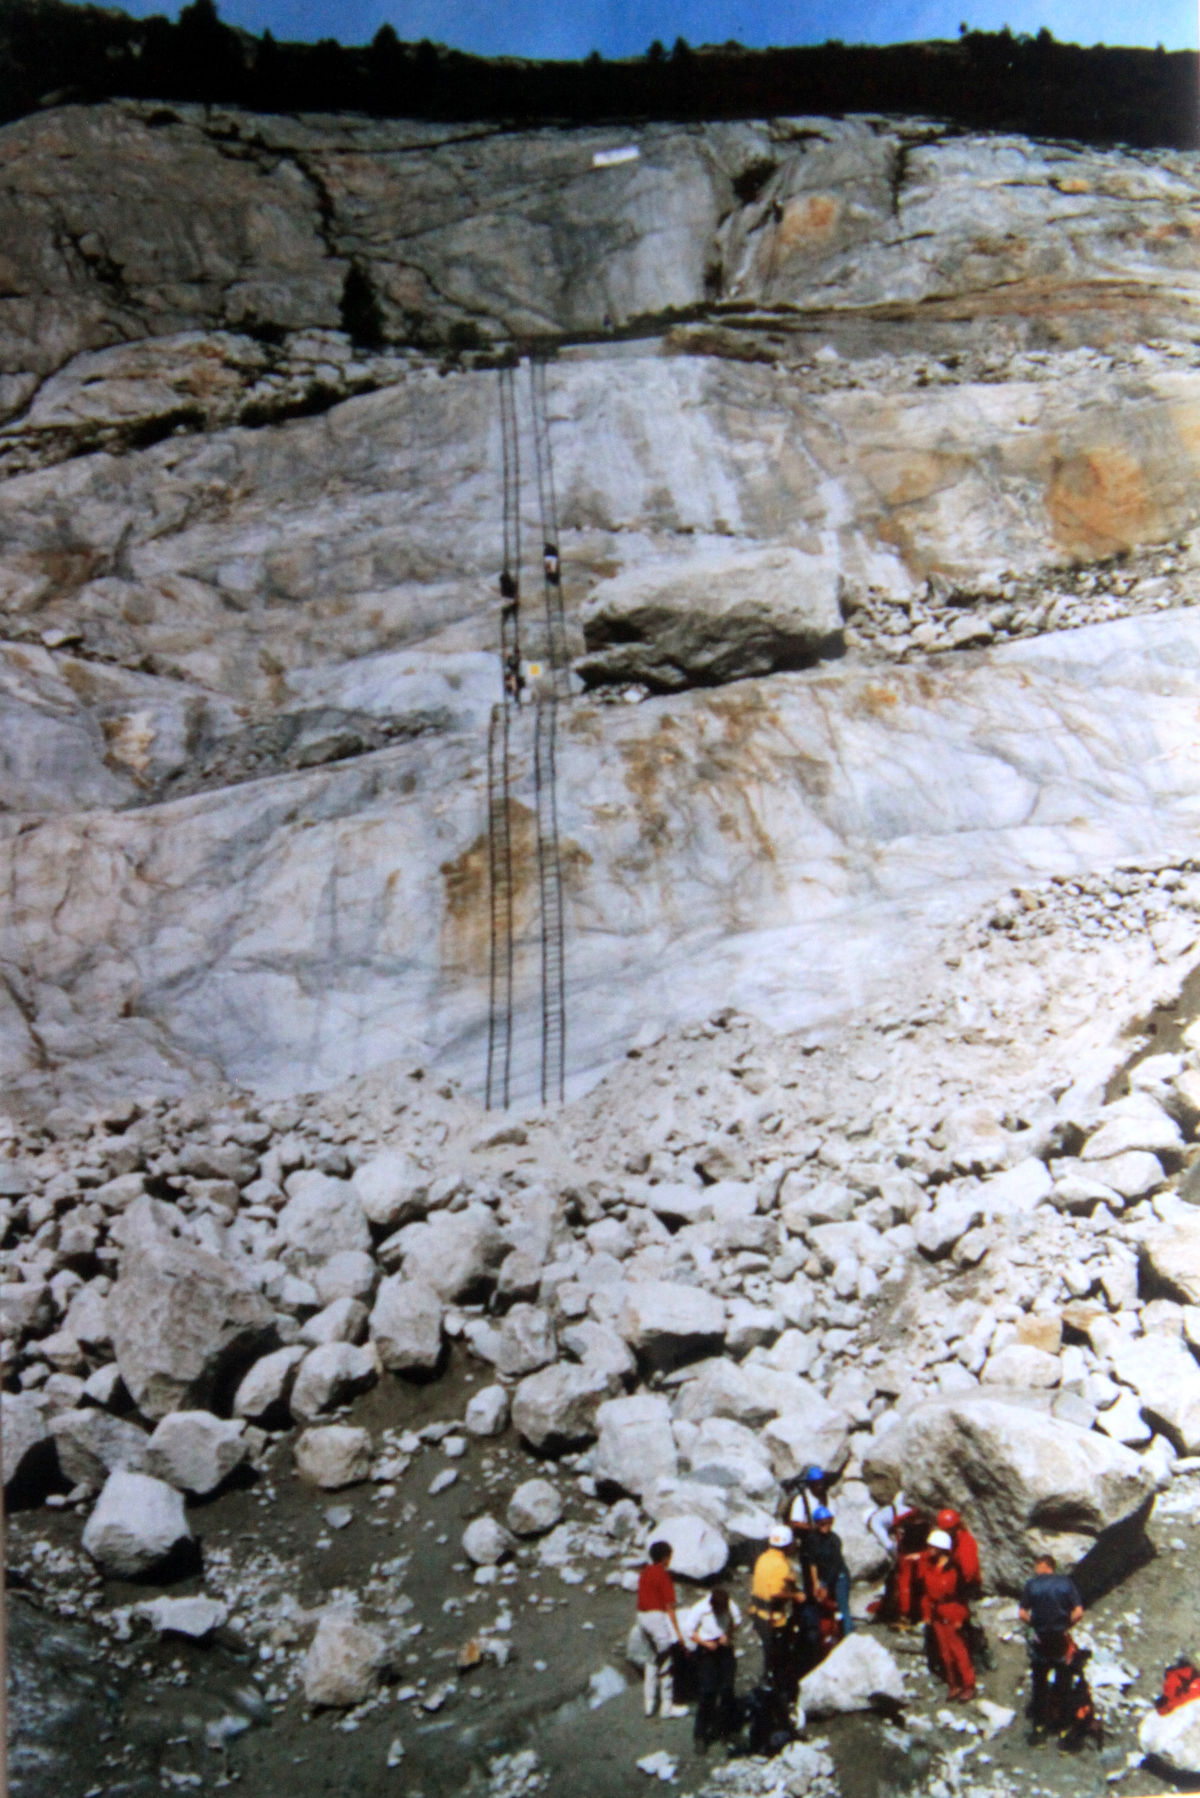
\includegraphics[width=0.49\linewidth]{\figs/balcons_1.JPG}
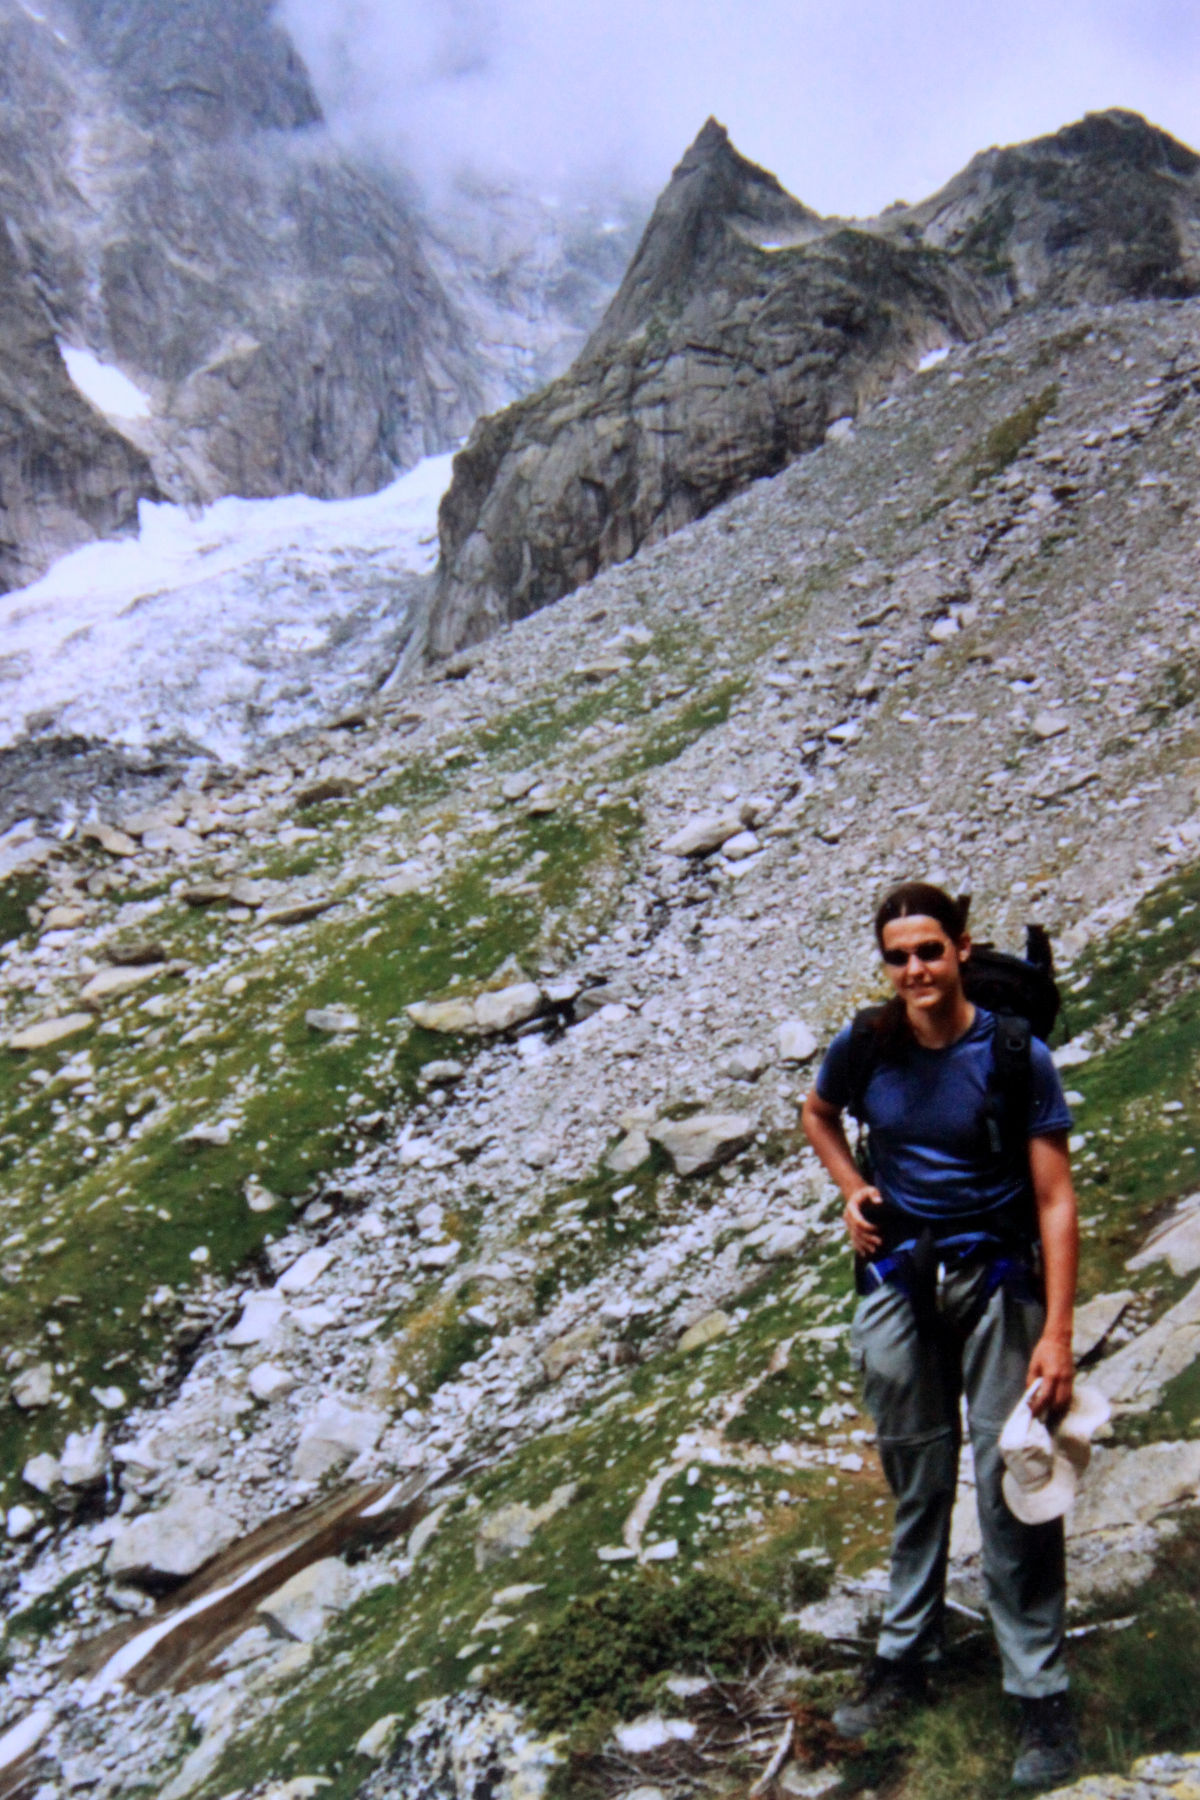
\includegraphics[width=0.49\linewidth]{\figs/balcons_2.JPG}
\textit{Left: the ladders leading to the Mer de Glace as in 2003. Right: the author in 2003. \\
Photos: Gilles Maussion}
\end{figure}

\chapter{Curriculum Vitae: Fabien Maussion}

\textit{Last updated: February 2021}

Department of Atmospheric and Cryospheric Science \\
Research centre for Climate \\
University of Innsbruck \\
Innrain 52f, A-6020 Innsbruck \\
Personal website: \href{https://fabienmaussion.info}{https://fabienmaussion.info}


\section*{Education}
\label{\detokenize{ch08/cv:education}}\begin{itemize}[nosep]
\item {} 
2002: Baccalaureate (High School Diploma)

\item {} 
2003--2004: Maths and physics preparation class in Strasbourg

\item {} 
2005--2006: \href{https://www.isae-supaero.fr/en/}{SUPAÉRO} -- Institut Supérieur de l’Aéronautique et de l’Espace, Toulouse (aerospace engineering school)

\item {} 
2007--2008: \href{https://www.tu.berlin/}{Technische Universität Berlin} -- International exchange year and Master degree

\item {} 
2008--2014: \href{https://www.klima.tu-berlin.de}{Technische Universität Berlin - Chair of Climatology} -- PhD thesis

\end{itemize}

\textbf{PhD Thesis} defended in February 2014 with the title “A new atmospheric dataset for High Asia: development,
validation and applications in climatology and in glaciology” (summa cum laude). 
Supervisor: Dieter Scherer. Reviewers: Christoph Schneider (RWTH Aachen), Georg Kaser (University of Innsbruck)


\section*{Professional experience}
\label{\detokenize{ch08/cv:professional-experience}}\begin{itemize}[nosep]
\item {} 
2006--2007: Interim year as engineering trainee -- Space mechanics at \href{https://www.c-s.fr}{C-S Group}, Toulouse

\item {} 
2008--2014: PhD / Post-doc at the \href{http://klima.tu-berlin.de}{Chair of Climatology}, Technische Universität Berlin

\item {} 
2014--2015: Post-doc at the Department of Atmospheric and Cryospheric Sciences (\href{https://www.uibk.ac.at/acinn}{ACINN}), Universität Innsbruck

\item {} 
2015--2016: University Assistant at \href{https://www.uibk.ac.at/acinn}{ACINN}, Universität Innsbruck

\item {} 
Since 2016: Assistant professor at \href{https://www.uibk.ac.at/acinn}{ACINN}, Universität Innsbruck

\end{itemize}


\section*{Research projects \& grants}
\label{\detokenize{ch08/cv:research-projects-grants}}
\textbf{As PI (current)}:
\begin{itemize}[nosep]
\item {} 
2021--2024: PROVIDE -- Paris Agreement Overshooting -- Reversibility, Climate Impacts and Adaptation Needs (H2020, 230k\texteuro{})

\item {} 
2019--2022: \href{https://agroclim-huaraz.info/}{AgroClim - Huaraz}, “Water availability and water demand in the Peruvian Andes” (ÖAW, 443k\texteuro{})

\item {} 
2020--2022: \href{https://www.uibk.ac.at/acinn/research/ice-and-climate/projects/scaling\_regional\_sea\_level\_changes.html.en}{Scaling regional sea-level changes with climate forcings} (FWF, Co-PI)

\end{itemize}

\textbf{As PI (completed)}:
\begin{itemize}[nosep]
\item {} 
2018--2021: \href{https://www.uibk.ac.at/acinn/research/ice-and-climate/projects/modelling-glacier-length-changes.html.en}{Modelling glacier length changes in Alps on the base of tree-ring based temperature reconstructions for the last 2500 years} (Universtität Innsbruck, 120k\texteuro{}, Co-PI)

\item {} 
2019--2020: “Glaciers on the Cloud: OGGM-Edu” (University of Innsbruck, 20k\texteuro{})

\item {} 
2018--2019: \href{https://www.uibk.ac.at/acinn/research/ice-and-climate/projects/holocene-climate-variability.html.en}{The Upper Grindelwald Glacier as indicator for Holocene climate variability} (TWF, 10k\texteuro{})

\end{itemize}

\textbf{As employee}:
\begin{itemize}[nosep]
\item {} 
2008--2014: \href{https://www.klima.tu-berlin.de/index.php?show=reg\_klima\_hochasien\_dynrgtip\&lan=en}{DynRG-TIP} -- Dynamic Response of Glaciers on the Tibetan Plateau to Climate Change (DFG)

\item {} 
2011--2014: \href{https://www.klima.tu-berlin.de/index.php?show=reg\_klima\_hochasien\_wet\&lan=en}{WET} -- Variability and Trends in Water Balance Components of Benchmark Drainage Basins on the Tibetan Plateau (BMBF)

\item {} 
2014--2015: \href{https://www.uibk.ac.at/acinn/research/ice-and-climate/projects/glaciation-of-tropical-mountains.html.en}{Multidecadal to Centennial Climate Variability: Assessing the Conditions for the Glaciation of Tropical Mountains} (FWF)

\end{itemize}


\section*{Awards}
\label{\detokenize{ch08/cv:awards}}\begin{itemize}[nosep]
\item {} 
Wilhelm-Lauer-Preis 2014 (Akademie der Wissenschaften und der Literatur, Mainz): Prize for an outstanding,
original dissertation in the field of mountain geography

\end{itemize}


\section*{Functions at the University of Innsbruck}
\label{\detokenize{ch08/cv:functions-at-the-university-of-innsbruck}}\begin{itemize}[nosep]
\item {} 
Deputy speaker (2017-2021) then speaker (2021-) of the Doctoral Programme “\href{https://www.uibk.ac.at/alpinerraum/dps/dp-mountainclimate/}{Mountain Climate and Environment}”

\item {} 
Chair of the “working group on IT and software infrastructure” at \href{https://www.uibk.ac.at/acinn}{ACINN}

\end{itemize}


\section*{Other activities \& services to the community}
\label{\detokenize{ch08/cv:other-activities-services-to-the-community}}\begin{itemize}[nosep]
\item {} 
Co-Chair of the IACS working group: \href{https://cryosphericsciences.org/activities/working-groups/rgi-working-group/}{Randolph Glacier Inventory (RGI) and its role in future glacier monitoring and GLIMS}

\item {} 
Member of the IACS working group: \href{https://cryosphericsciences.org/activities/ice-thickness/}{Glacier ice thickness estimation}

\item {} 
Member of the CLIC working group: \href{http://www.climate-cryosphere.org/mips/glaciermip}{Glacier Model Intercomparison Project}

\item {} 
Scientific editor: \href{https://www.geosci-model-dev.net/}{Geoscientific Model Development} (EGU Journal)

\item {} 
Reviewer: \textit{J. Geophys. Res., J. Hydrometeorol., Int. J. Climatol., J. Hydrol., The Cryosph., J. Glaciol., Hydrol. Earth Syst. Sci., Q.J.R. Meteorol. Soc., Earth Syst. Dynam., …}

\end{itemize}


\section*{Contributions to open source software and open data}
\label{\detokenize{ch08/cv:contributions-to-open-source-software-and-open-data}}\begin{itemize}[nosep]
\item {} 
\href{http://oggm.org}{oggm.org} (2016-present): glacier evolution model

\item {} 
\href{http://edu.oggm.org}{edu.oggm.org} (2019-present): educational platform

\item {} 
\href{http://xarray.pydata.org}{xarray} (2015-2018): array manipulation software

\item {} 
\href{https://salem.readthedocs.io}{salem} (2014-present): map visualization and WRF model analysis software

\item {} 
\href{https://www.klima.tu-berlin.de/HAR}{High Asia Refined analysis (HAR)}: atmospheric dataset

\item {} 
\href{https://rgitools.readthedocs.io/en/latest/dems.html}{RGI-TOPO}: topography dataset for mountain glaciers

\item {} 
…

\end{itemize}


\section*{Teaching}
\label{\detokenize{ch08/cv:teaching}}
\textit{Current teaching load: 8 hours per week in the winter term.}

\textbf{Current classes}
\begin{itemize}[nosep]
\item {} 
\textbf{Introduction to meteorology and climatology}:
\href{https://orawww.uibk.ac.at/public/lfuonline\_lv.details?sem\_id\_in=16W\&lvnr\_id\_in=707606}{fundamentals of the climate system}
for undergraduate students (winter semester, 2hrs).

Topics: components of the
climate system, general circulation of the atmosphere and of the oceans,
climate variability (ENSO, NAO, Monsoon), climate change and climate policy.

\item {} 
\textbf{Physics of the climate system}: \href{https://orawww.uibk.ac.at/public/lfuonline\_lv.details?sem\_id\_in=15W\&lvnr\_id\_in=707712}{advanced course in physical climatology}
for graduate students (winter semester, 3hrs).

Climate variability, synoptic climatology, paleoclimate, climate modelling,
climate change and feedbacks.

The lecture practicals are \href{http://fabienmaussion.info/climate\_system/}{available online}.

\item {} 
\textbf{Scientific Programming}: \href{https://orawww.uibk.ac.at/public/lfuonline\_lv.details?sem\_id\_in=18S\&lvnr\_id\_in=707716}{advanced course in programming}
for graduate students (winter semester, 3hrs).

Modern programming techniques for (geo-)scientists:
numerics, software structure, unit testing, object-oriented programming, version control, open development practices…

The lecture notes are \href{http://fabienmaussion.info/scientific\_programming/}{available online}.

\end{itemize}

Most recent student evaluations (2020/21):
\href{https://fabienmaussion.info/images/teaching/eval/2020WS\_SciPro.pdf}{scientific programming},
\href{https://fabienmaussion.info/images/teaching/eval/2020WS\_PhyClim.pdf}{physics of the climate system},
\href{https://fabienmaussion.info/images/teaching/eval/2020WS\_EKlim.pdf}{Einführung in die Klimatologie}.

\textbf{Past classes}

For a full list of past classes and student evaluations, visit \href{https://fabienmaussion.info/teaching/}{my personal website}.


\section*{Student supervision}
\label{\detokenize{ch08/cv:student-supervision}}

\subsection*{PhD theses (completed)}
\label{\detokenize{ch08/cv:phd-theses-completed}}\begin{itemize}[nosep]
\item {} 
\textbf{Julia Eis} (Universität Bremen, co-supervised, 2020)
: Reconstructing glacier evolution using a flowline model (\href{https://media.suub.uni-bremen.de/handle/elib/4635}{link})

\item {} 
\textbf{Beatriz Recinos} (Universität Bremen, co-supervised, 2020)
: Ocean-glacier interaction on the large regional scale (\href{https://media.suub.uni-bremen.de/handle/elib/4637}{link})

\end{itemize}


\subsection*{Master theses (completed)}
\label{\detokenize{ch08/cv:master-theses-completed}}\begin{itemize}[nosep]
\item {} 
\textbf{Castellani, M.} (ACINN, 2020)
: Estimating Glacier Ice Thickness with Machine Learning (\href{https://diglib.uibk.ac.at/urn:nbn:at:at-ubi:1-60115}{link})

\item {} 
\textbf{Schuster, L.} (ACINN, 2020)
: Response time sensitivity of glaciers using the Open Global Glacier Model (\href{https://diglib.uibk.ac.at/ulbtirolhs/content/titleinfo/4864453}{link})

\item {} 
\textbf{Trichtl, M.} (ACINN, 2020)
: The atmospheric water budget over the Tibetan Plateau in ERA-Interim and ERA5 reanalyses (\href{https://diglib.uibk.ac.at/ulbtirolhs/content/titleinfo/4888002}{link})

\item {} 
\textbf{Hatvan, V.} (ACINN, 2019)
: Evaluation of the physical SNOWPACK model under arctic conditions : An applicability study for the area around Longyearbyen, Svalbard (\href{http://diglib.uibk.ac.at/ulbtirolhs/content/titleinfo/3584652}{link})

\item {} 
\textbf{Gregor, P.} (ACINN, 2019)
: Inversion of Glacier Bed from Surface Observations by Cost Minimization : Introducing the Open Source Model COMBINE (\href{http://diglib.uibk.ac.at/ulbtirolhs/content/titleinfo/3086935}{link})

\item {} 
\textbf{Kilian, M.} (ACINN @ DLR, co-supervised, 2018)
: Impact of the Eruption of Mt. Pinatubo on the chemical composition of the tropical atmosphere as simulated with EMAC

\item {} 
\textbf{Cerny, M.} (ACINN, 2018)
: Lake-level changes on the Tibetan Plateau and their Relation to Glacial Melt (\href{http://diglib.uibk.ac.at/ulbtirolhs/content/titleinfo/2347464}{link})

\item {} 
\textbf{Schlumpberger, M.} (ACINN, 2017)
: Wet and dry spells in the Rio Santa Basin, Peruvian Andes, and connections to the large-scale circulation (\href{http://diglib.uibk.ac.at/urn:nbn:at:at-ubi:1-6985}{link})

\item {} 
\textbf{Siller, M.} (ACINN, 2017)
: WRF simulation of wet and dry spells in the Rio Santa Basin, Peruvian Andes - A WRF Modeling Case Study (\href{http://diglib.uibk.ac.at/urn:nbn:at:at-ubi:1-7816}{link})

\item {} 
\textbf{Thorlaksson, D.} (ACINN, 2017)
: Calibrating a glacier ice thickness model from in-situ point measurements (\href{http://diglib.uibk.ac.at/urn:nbn:at:at-ubi:1-7259}{link})

\item {} 
\textbf{Zier, C.} (ACINN, co-supervised, 2017)
: Wie beeinflussen großskalige Wetterstrukturen das lokale Wetter in den Anden von Chile? Ein Downscaling Experiment (\href{http://diglib.uibk.ac.at/urn:nbn:at:at-ubi:1-7092}{link})

\item {} 
\textbf{Zolles, T.} (ACINN, 2016)
: Uncertainty estimation of a glacier mass balance model (\href{http://diglib.uibk.ac.at/urn:nbn:at:at-ubi:1-5240}{link})

\end{itemize}


\subsection*{Bachelor theses (completed)}
\label{\detokenize{ch08/cv:bachelor-theses-completed}}\begin{itemize}[nosep]
\item {} 
\textbf{Schwienbacher, F.} (ACINN, 2017)
: Model sensitivity of the mass balance module of the \href{http://oggm.org/}{OGGM} model

\item {} 
\textbf{Oberrauch, M.} (ACINN, 2016)
: Calibration and validation of a glacier model applied to the Upper Grindelwald Glacier from 1880 to present

\item {} 
\textbf{Gstir, T.}  (ACINN, 2016)
: Klimasensitivität des Oberen Grindelwaldgletschers untersucht mithilfe des \href{http://oggm.org}{OGGM}

\end{itemize}

For a list of current advisees, visit \href{https://fabienmaussion.info/team/}{my personal website}.


\clearpage

\section*{List of publications - Fabien Maussion}

\begin{footnotesize}
\begin{itemize}[nosep]
\item {} 
Schuster, L., Maussion, F., Langhamer, L. and Moseley, G. E.: Lagrangian detection of precipitation moisture sources
for an arid region in northeast Greenland: relations to the North Atlantic Oscillation, sea ice cover, and temporal
trends from 1979 to 2017, Weather Clim. Dyn., 2(1), 1--17, doi:10.5194/wcd-2-1-2021, 2021.

\item {} 
Marzeion, B., Hock, R., Anderson, B., Bliss, A., Champollion, N., Fujita, K., Huss, M., Immerzeel, W., Kraaijenbrink,
P., Malles, J., Maussion, F., Radić, V., Rounce, D. R., Sakai, A., Shannon, S., Wal, R. and Zekollari, H.:
Partitioning the Uncertainty of Ensemble Projections of Global Glacier Mass Change, Earth’s Futur., 8(7), doi:
10.1029/2019ef001470, 2020.

\item {} 
Pelto, B. M., Maussion, F., Menounos, B., Radić, V. and Zeuner, M.: Bias-corrected estimates of glacier thickness in
the Columbia River Basin, Canada, J. Glaciol., 1--13, doi:10.1017/jog.2020.75, 2020.

\item {} 
Zemp, M., Huss, M., Thibert, E., Eckert, N., McNabb, R., Huber, J., Barandun, M., Machguth, H., Nussbaumer, S. U.,
Gärtner-Roer, I., Thomson, L., Paul, F., Maussion, F., Kutuzov, S. and Cogley, J. G.: Global glacier mass changes and
their contributions to sea-level rise from 1961 to 2016, Nature, 568(7752), 382--386, doi:10.1038/s41586-019-1071-0,
2019.

\item {} 
Recinos, B., Maussion, F., Rothenpieler, T. and Marzeion, B.: Impact of frontal ablation on the ice thickness
estimation of marine-terminating glaciers in Alaska, Cryosph., 13(10), 2657--2672, doi:10.5194/tc-13-2657-2019, 2019.

\item {} 
Maussion, F., Butenko, A., Champollion, N., Dusch, M., Eis, J., Fourteau, K., Gregor, P., Jarosch, A. H., Landmann,
J., Oesterle, F., Recinos, B., Rothenpieler, T., Vlug, A., Wild, C. T. and Marzeion, B.: The Open Global Glacier
Model (OGGM) v1.1, Geosci. Model Dev., 12(3), 909--931, doi:10.5194/gmd-12-909-2019, 2019.

\item {} 
Horak, J., Hofer, M., Maussion, F., Gutmann, E., Gohm, A. and Rotach, M. W.: Assessing the added value of the
Intermediate Complexity Atmospheric Research (ICAR) model for precipitation in complex topography, Hydrol. Earth Syst.
Sci., 23(6), 2715--2734, doi:10.5194/hess-23-2715-2019, 2019.

\item {} 
Eis, J., Maussion, F. and Marzeion, B.: Initialization of a global glacier model based on present-day glacier geometry
and past climate information: an ensemble approach, Cryosph., 13(12), 3317--3335, doi:10.5194/tc-13-3317-2019, 2019.

\item {} 
Zolles, T., Maussion, F., Galos, S. P., Gurgiser, W. and Nicholson, L.: Robust uncertainty assessment of the
spatio-temporal transferability of glacier mass and energy balance models, Cryosph., 13(2), 469--489, doi:
10.5194/tc-13-469-2019, 2019.

\item {} 
Farinotti, D., Huss, M., Fürst, J. J., Landmann, J., Machguth, H., Maussion, F. and Pandit, A.: A consensus estimate
for the ice thickness distribution of all glaciers on Earth, Nat. Geosci., 12(3), 168--173, doi:
10.1038/s41561-019-0300-3, 2019.

\item {} 
Strasser, U., Marke, T., Braun, L., Escher-Vetter, H., Juen, I., Kuhn, M., Maussion, F., Mayer, C., Nicholson, L.,
Niedertscheider, K., Sailer, R., Stötter, J., Weber, M. and Kaser, G.: The Rofental: a high Alpine research basin (
1890--3770 m a.s.l.) in the Ötztal Alps (Austria) with over 150 years of hydrometeorological and glaciological
observations, Earth Syst. Sci. Data, 10(1), 151--171, doi:10.5194/essd-10-151-2018, 2018.

\item {} 
Goosse, H., Barriat, P.-Y., Dalaiden, Q., Klein, F., Marzeion, B., Maussion, F., Pelucchi, P. and Vlug, A.: Testing
the consistency between changes in simulated climate and Alpine glacier length over the past millennium, Clim. Past,
14(8), 1119--1133, doi:10.5194/cp-14-1119-2018, 2018.

\item {} 
Marzeion, B., Kaser, G., Maussion, F. and Champollion, N.: Limited influence of climate change mitigation on
short-term glacier mass loss, Nat. Clim. Chang., 8, doi:10.1038/s41558-018-0093-1, 2018.

\item {} 
Mölg, T., Maussion, F., Collier, E., Chiang, J. C. H. and Scherer, D.: Prominent mid-latitude circulation signature in
High Asia’s surface climate during monsoon, J. Geophys. Res. Atmos., 1--11, doi:10.1002/2017JD027414, 2017.

\item {} 
Galos, S. P., Klug, C., Maussion, F., Covi, F., Nicholson, L., Rieg, L., Gurgiser, W., Mölg, T. and Kaser, G.:
Reanalysis of a 10-year record (2004--2013) of seasonal mass balances at Langenferner/Vedretta Lunga, Ortler Alps,
Italy, Cryosph., 11(3), 1417--1439, doi:10.5194/tc-11-1417-2017, 2017.

\item {} 
Farinotti, D., Brinkerhoff, D. J., Clarke, G. K. C., Fürst, J. J., Frey, H., Gantayat, P., Gillet-Chaulet, F., Girard,
C., Huss, M., Leclercq, P. W., Linsbauer, A., Machguth, H., Martin, C., Maussion, F., Morlighem, M., Mosbeux, C.,
Pandit, A., Portmann, A., Rabatel, A., Ramsankaran, R., Reerink, T. J., Sanchez, O., Stentoft, P. A., Singh Kumari,
S., van Pelt, W. J. J., Anderson, B., Benham, T., Binder, D., Dowdeswell, J. A., Fischer, A., Helfricht, K., Kutuzov,
S., Lavrentiev, I., McNabb, R., Gudmundsson, G. H., Li, H. and Andreassen, L. M.: How accurate are estimates of
glacier ice thickness? Results from ITMIX, the Ice Thickness Models Intercomparison eXperiment, Cryosph., 11(2),
949--970, doi:10.5194/tc-11-949-2017, 2017.

\item {} 
Spiess, M., Schneider, C. and Maussion, F.: MODIS-derived interannual variability of the equilibrium-line altitude
across the Tibetan Plateau, Ann. Glaciol., 57(71), 140--154, doi:10.3189/2016AoG71A014, 2016.

\item {} 
Otto, M., Höpfner, C., Curio, J., Maussion, F. and Scherer, D.: Assessing vegetation response to precipitation in
northwest Morocco during the last decade: an application of MODIS NDVI and high resolution reanalysis data, Theor.
Appl. Climatol., 123(1--2), 23--41, doi:10.1007/s00704-014-1344-3, 2016.

\item {} 
Biskop, S., Maussion, F., Krause, P. and Fink, M.: Differences in the water-balance components of four lakes in the
southern-central Tibetan Plateau, Hydrol. Earth Syst. Sci, 20, 209--225, doi:10.5194/hess-20-209-2016, 2016.

\item {} 
Zhu, M., Yao, T., Yang, W., Maussion, F., Huintjes, E. and Li, S.: Energy- and mass-balance comparison between Zhadang
and Parlung No. 4 glaciers on the Tibetan Plateau, J. Glaciol., 61(227), 595--607, \\ doi:10.3189/2015JoG14J206, 2015.

\item {} 
Spiess, M., Maussion, F., Möller, M., Scherer, D. and Schneider, C.: Modis derived equilibrium line altitude estimates
for purogangri ice cap, tibetan plateau, and their relation to climatic predictors (2001--2012), Geogr. Ann. Ser. A,
Phys. Geogr., 97(3), 599--614, doi:10.1111/geoa.12102, 2015.

\item {} 
Huintjes, E., Sauter, T., Schröter, B., Maussion, F., Yang, W., Kropáček, J., Buchroithner, M., Scherer, D., Kang, S.
and Schneider, C.: Evaluation of a Coupled Snow and Energy Balance Model for Zhadang Glacier, Tibetan Plateau, Using
Glaciological Measurements and Time-Lapse Photography, Arctic, Antarct. Alp. Res., 47(3), 573--590, doi:
10.1657/AAAR0014-073, 2015.

\item {} 
Curio, J., Maussion, F. and Scherer, D.: A 12-year high-resolution climatology of atmospheric water transport over the
Tibetan Plateau, Earth Syst. Dyn., 6(1), 109--124, doi:10.5194/esd-6-109-2015, 2015.

\item {} 
Collier, E., Maussion, F., Nicholson, L. I., Mölg, T., Immerzeel, W. W. and Bush, a. B. G.: Impact of debris cover on
glacier ablation and atmosphere--glacier feedbacks in the Karakoram, Cryosph., 9(4), 1617--1632, doi:
10.5194/tc-9-1617-2015, 2015.

\item {} 
Maussion, F., Gurgiser, W., Großhauser, M., Kaser, G. and Marzeion, B.: ENSO influence on surface energy and mass
balance at Shallap Glacier, Cordillera Blanca, Peru, Cryosph., 9(4), 1663--1683, doi:10.5194/tc-9-1663-2015, 2015.

\item {} 
Mölg, T., Maussion, F. and Scherer, D.: Mid-latitude westerlies as a driver of glacier variability in monsoonal High
Asia, Nat. Clim. Chang., 4(1), 68--73, doi:10.1038/nclimate2055, 2014.

\item {} 
Maussion, F., Scherer, D., Mölg, T., Collier, E., Curio, J. and Finkelnburg, R.: Precipitation Seasonality and
Variability over the Tibetan Plateau as Resolved by the High Asia Reanalysis*, J. Clim., 27(5), 1910--1927, doi:
10.1175/JCLI-D-13-00282.1, 2014.

\item {} 
Dietze, E., Maussion, F., Ahlborn, M., Diekmann, B., Hartmann, K., Henkel, K., Kasper, T., Lockot, G., Opitz, S. and
Haberzettl, T.: Sediment transport processes across the Tibetan Plateau inferred from robust grain-size end members in
lake sediments, Clim. Past, 10(1), 91--106, doi:10.5194/cp-10-91-2014, 2014.

\item {} 
Collier, E., Nicholson, L. I., Brock, B. W., Maussion, F., Essery, R. and Bush, a. B. G.: Representing moisture fluxes
and phase changes in glacier debris cover using a reservoir approach, Cryosph., 8(4), 1429--1444, doi:
10.5194/tc-8-1429-2014, 2014.

\item {} 
Kropacek, J., Maussion, F., Chen, F., Hoerz, S., Hochschild, V. and Kropáček, J.: Analysis of ice phenology of lakes
on the Tibetan Plateau from MODIS data, Cryosph., 7(1), 287--301, doi:10.5194/tc-7-287-2013, 2013.

\item {} 
Collier, E., Mölg, T., Maussion, F., Scherer, D., Mayer, C. and Bush, a. B. G.: High-resolution interactive modelling
of the mountain glacier--atmosphere interface: an application over the Karakoram, Cryosph., 7(3), 779--795, doi:
10.5194/tc-7-779-2013, 2013.

\item {} 
Mölg, T., Maussion, F., Yang, W. and Scherer, D.: The footprint of Asian monsoon dynamics in the mass and energy
balance of a Tibetan glacier, Cryosph., 6(6), 1445--1461, doi:10.5194/tc-6-1445-2012, 2012.

\item {} 
Maussion, F., Scherer, D., Finkelnburg, R., Richters, J., Yang, W. and Yao, T.: WRF simulation of a precipitation
event over the Tibetan Plateau, China -- an assessment using remote sensing and ground observations, Hydrol. Earth
Syst. Sci., 15(6), 1795--1817, doi:10.5194/hess-15-1795-2011, 2011.

\item {} 
Bolch, T., Yao, T., Kang, S., Buchroithner, M. F., Scherer, D., Maussion, F., Huintjes, E. and Schneider, C.: A
glacier inventory for the western Nyainqentanglha Range and the Nam Co Basin, Tibet, and glacier changes 1976-2009,
Cryosph., 4(3), 419--433, doi:10.5194/tc-4-419-2010, 2010.


\end{itemize}
\end{footnotesize}


%\input{./chapters/chapter1}
%\input{./chapters/chapter2}
%\input{./chapters/chapter3}
%\input{./chapters/chapter4}
%\input{./chapters/chapter5}
%\input{./chapters/chapter6}
%\input{./chapters/chapter7}
%\input{./chapters/chapter8}

%\input{./papers/paper1}
%\input{./papers/paper2}
%\input{./papers/paper3}
%\input{./papers/paper4}
%\input{./papers/paper5}

\begin{footnotesize}
\cleardoublepage\phantomsection
\bibliographystyle{copernicus}
\bibliography{../habil/references}
\end{footnotesize}

\end{document}
